% Options for packages loaded elsewhere
\PassOptionsToPackage{unicode}{hyperref}
\PassOptionsToPackage{hyphens}{url}
%
\documentclass[
  man,floatsintext]{apa6}
\usepackage{amsmath,amssymb}
\usepackage{iftex}
\ifPDFTeX
  \usepackage[T1]{fontenc}
  \usepackage[utf8]{inputenc}
  \usepackage{textcomp} % provide euro and other symbols
\else % if luatex or xetex
  \usepackage{unicode-math} % this also loads fontspec
  \defaultfontfeatures{Scale=MatchLowercase}
  \defaultfontfeatures[\rmfamily]{Ligatures=TeX,Scale=1}
\fi
\usepackage{lmodern}
\ifPDFTeX\else
  % xetex/luatex font selection
\fi
% Use upquote if available, for straight quotes in verbatim environments
\IfFileExists{upquote.sty}{\usepackage{upquote}}{}
\IfFileExists{microtype.sty}{% use microtype if available
  \usepackage[]{microtype}
  \UseMicrotypeSet[protrusion]{basicmath} % disable protrusion for tt fonts
}{}
\makeatletter
\@ifundefined{KOMAClassName}{% if non-KOMA class
  \IfFileExists{parskip.sty}{%
    \usepackage{parskip}
  }{% else
    \setlength{\parindent}{0pt}
    \setlength{\parskip}{6pt plus 2pt minus 1pt}}
}{% if KOMA class
  \KOMAoptions{parskip=half}}
\makeatother
\usepackage{xcolor}
\usepackage{graphicx}
\makeatletter
\def\maxwidth{\ifdim\Gin@nat@width>\linewidth\linewidth\else\Gin@nat@width\fi}
\def\maxheight{\ifdim\Gin@nat@height>\textheight\textheight\else\Gin@nat@height\fi}
\makeatother
% Scale images if necessary, so that they will not overflow the page
% margins by default, and it is still possible to overwrite the defaults
% using explicit options in \includegraphics[width, height, ...]{}
\setkeys{Gin}{width=\maxwidth,height=\maxheight,keepaspectratio}
% Set default figure placement to htbp
\makeatletter
\def\fps@figure{htbp}
\makeatother
\setlength{\emergencystretch}{3em} % prevent overfull lines
\providecommand{\tightlist}{%
  \setlength{\itemsep}{0pt}\setlength{\parskip}{0pt}}
\setcounter{secnumdepth}{-\maxdimen} % remove section numbering
% Make \paragraph and \subparagraph free-standing
\ifx\paragraph\undefined\else
  \let\oldparagraph\paragraph
  \renewcommand{\paragraph}[1]{\oldparagraph{#1}\mbox{}}
\fi
\ifx\subparagraph\undefined\else
  \let\oldsubparagraph\subparagraph
  \renewcommand{\subparagraph}[1]{\oldsubparagraph{#1}\mbox{}}
\fi
\newlength{\cslhangindent}
\setlength{\cslhangindent}{1.5em}
\newlength{\csllabelwidth}
\setlength{\csllabelwidth}{3em}
\newlength{\cslentryspacingunit} % times entry-spacing
\setlength{\cslentryspacingunit}{\parskip}
\newenvironment{CSLReferences}[2] % #1 hanging-ident, #2 entry spacing
 {% don't indent paragraphs
  \setlength{\parindent}{0pt}
  % turn on hanging indent if param 1 is 1
  \ifodd #1
  \let\oldpar\par
  \def\par{\hangindent=\cslhangindent\oldpar}
  \fi
  % set entry spacing
  \setlength{\parskip}{#2\cslentryspacingunit}
 }%
 {}
\usepackage{calc}
\newcommand{\CSLBlock}[1]{#1\hfill\break}
\newcommand{\CSLLeftMargin}[1]{\parbox[t]{\csllabelwidth}{#1}}
\newcommand{\CSLRightInline}[1]{\parbox[t]{\linewidth - \csllabelwidth}{#1}\break}
\newcommand{\CSLIndent}[1]{\hspace{\cslhangindent}#1}
\ifLuaTeX
\usepackage[bidi=basic]{babel}
\else
\usepackage[bidi=default]{babel}
\fi
\babelprovide[main,import]{english}
% get rid of language-specific shorthands (see #6817):
\let\LanguageShortHands\languageshorthands
\def\languageshorthands#1{}
% Manuscript styling
\usepackage{upgreek}
\captionsetup{font=singlespacing,justification=justified}

% Table formatting
\usepackage{longtable}
\usepackage{lscape}
% \usepackage[counterclockwise]{rotating}   % Landscape page setup for large tables
\usepackage{multirow}		% Table styling
\usepackage{tabularx}		% Control Column width
\usepackage[flushleft]{threeparttable}	% Allows for three part tables with a specified notes section
\usepackage{threeparttablex}            % Lets threeparttable work with longtable

% Create new environments so endfloat can handle them
% \newenvironment{ltable}
%   {\begin{landscape}\centering\begin{threeparttable}}
%   {\end{threeparttable}\end{landscape}}
\newenvironment{lltable}{\begin{landscape}\centering\begin{ThreePartTable}}{\end{ThreePartTable}\end{landscape}}

% Enables adjusting longtable caption width to table width
% Solution found at http://golatex.de/longtable-mit-caption-so-breit-wie-die-tabelle-t15767.html
\makeatletter
\newcommand\LastLTentrywidth{1em}
\newlength\longtablewidth
\setlength{\longtablewidth}{1in}
\newcommand{\getlongtablewidth}{\begingroup \ifcsname LT@\roman{LT@tables}\endcsname \global\longtablewidth=0pt \renewcommand{\LT@entry}[2]{\global\advance\longtablewidth by ##2\relax\gdef\LastLTentrywidth{##2}}\@nameuse{LT@\roman{LT@tables}} \fi \endgroup}

% \setlength{\parindent}{0.5in}
% \setlength{\parskip}{0pt plus 0pt minus 0pt}

% Overwrite redefinition of paragraph and subparagraph by the default LaTeX template
% See https://github.com/crsh/papaja/issues/292
\makeatletter
\renewcommand{\paragraph}{\@startsection{paragraph}{4}{\parindent}%
  {0\baselineskip \@plus 0.2ex \@minus 0.2ex}%
  {-1em}%
  {\normalfont\normalsize\bfseries\itshape\typesectitle}}

\renewcommand{\subparagraph}[1]{\@startsection{subparagraph}{5}{1em}%
  {0\baselineskip \@plus 0.2ex \@minus 0.2ex}%
  {-\z@\relax}%
  {\normalfont\normalsize\itshape\hspace{\parindent}{#1}\textit{\addperi}}{\relax}}
\makeatother

% \usepackage{etoolbox}
\makeatletter
\patchcmd{\HyOrg@maketitle}
  {\section{\normalfont\normalsize\abstractname}}
  {\section*{\normalfont\normalsize\abstractname}}
  {}{\typeout{Failed to patch abstract.}}
\patchcmd{\HyOrg@maketitle}
  {\section{\protect\normalfont{\@title}}}
  {\section*{\protect\normalfont{\@title}}}
  {}{\typeout{Failed to patch title.}}
\makeatother

\usepackage{xpatch}
\makeatletter
\xapptocmd\appendix
  {\xapptocmd\section
    {\addcontentsline{toc}{section}{\appendixname\ifoneappendix\else~\theappendix\fi\\: #1}}
    {}{\InnerPatchFailed}%
  }
{}{\PatchFailed}
\keywords{punishment; cooperation; economic games\newline\indent Word count: 5185 words}
\usepackage{lineno}

\linenumbers
\usepackage{csquotes}
\usepackage{array}
\usepackage{caption}
\usepackage{graphicx}
\usepackage{siunitx}
\usepackage[normalem]{ulem}
\usepackage{colortbl}
\usepackage{multirow}
\usepackage{hhline}
\usepackage{calc}
\usepackage{tabularx}
\usepackage{threeparttable}
\usepackage{wrapfig}
\usepackage{adjustbox}
\usepackage{hyperref}
\usepackage{setspace}
\usepackage{amsmath}
\usepackage{xcolor}
\usepackage{makecell}
\raggedbottom
\AtBeginEnvironment{tabular}{\singlespacing}
\AtBeginEnvironment{lltable}{\singlespacing}
\AtBeginEnvironment{tablenotes}{\doublespacing}
\captionsetup[table]{font={stretch=1,small}}
\captionsetup[figure]{font={stretch=1,small}}
\nolinenumbers
\note{\raggedright * Correspondence concerning this article should be addressed to Scott Claessens, Level 2, Building 302, 23 Symonds Street, Auckland, New Zealand. \text{E-mail:} \href{scott.claessens@gmail.com}{\nolinkurl{scott.claessens@gmail.com}} \par This working paper has not yet been peer-reviewed.}
\ifLuaTeX
  \usepackage{selnolig}  % disable illegal ligatures
\fi
\IfFileExists{bookmark.sty}{\usepackage{bookmark}}{\usepackage{hyperref}}
\IfFileExists{xurl.sty}{\usepackage{xurl}}{} % add URL line breaks if available
\urlstyle{same}
\hypersetup{
  pdftitle={Why do people punish? Evidence for a range of strategic concerns},
  pdfauthor={Scott Claessens*1, Quentin D. Atkinson1, \& Nichola Raihani1,2},
  pdflang={en-EN},
  pdfkeywords={punishment; cooperation; economic games},
  hidelinks,
  pdfcreator={LaTeX via pandoc}}

\title{Why do people punish? Evidence for a range of strategic concerns}
\author{Scott Claessens\textsuperscript{*1}, Quentin D. Atkinson\textsuperscript{1}, \& Nichola Raihani\textsuperscript{1,2}}
\date{}


\shorttitle{Punishment strategies}

\affiliation{\vspace{0.5cm}\textsuperscript{1} \footnotesize School of Psychology, University of Auckland, Auckland, New Zealand\\\textsuperscript{2} \footnotesize Department of Experimental Psychology, University College London, London, United Kingdom}

\abstract{%
Costly punishment is thought to be one of the key mechanisms sustaining cooperation in humans. However, the motives for punitive behaviour remain unclear. Punishment is often assumed to be motivated by a desire to convert free riders into cooperators, but it is also consistent with a host of other functions, such as levelling payoffs or increasing one's relative position. We used a suite of six economic games to tease apart the different motives for punishment. Across representative samples from the United Kingdom and the United States, we estimated the frequency of different punishment strategies in the population, finding that egalitarian motives for punishment are more common than behaviour-change motives. Moreover, different punishment strategies were differentially predicted by personality, social preferences, political ideology, and religious views. Self-reports of behaviour in the games suggested that people have some degree of insight into their punishment strategy. These findings highlight the multipurpose nature of human punishment.
}



\begin{document}
\maketitle

\linenumbers

\hypertarget{introduction}{%
\section{Introduction}\label{introduction}}

Humans cooperate on a scale that is unparalleled in the animal kingdom. One
mechanism thought to sustain this level of cooperation is costly punishment,
whereby individuals harm others at a personal cost\textsuperscript{1},
ostensibly encouraging cooperative behaviour from the target (or bystanders\textsuperscript{2--4}) in the future. Punishment
therefore offers a route to maintaining or increasing cooperation by changing
the payoff structure of social interactions such that it no longer pays to cheat
or exploit social partners\textsuperscript{1,5}.

In humans, many studies of punishment have been carried out in laboratory
settings using economic games\textsuperscript{6--15}. In these games, participants are usually given a sum of money
that they can use to invest in collective action or to help others.
Alternatively, participants can `cheat' by keeping the money for themselves or
by exploiting the contributions of others. Punishment is introduced into such
games by giving participants the option to pay a small `fee' to impose a greater
`fine' on their co-players. Several lines of experimental evidence indicate that
people use this punishment option\textsuperscript{12}, that they enjoy
punishing\textsuperscript{16}, and that they frequently, though not
always\textsuperscript{17}, punish cheating or exploitative
co-players\textsuperscript{10,11}.

Evidence from these experiments suggests that the threat of costly punishment
plays an important role in promoting human cooperation. People tend to cooperate
more in games where punishment is possible compared to those where it is not\textsuperscript{6,7,15}. The effect that the threat of
punishment has on cooperation is also evident in the higher contributions
typically observed in the Ultimatum Game (where punishment is possible) compared
to the structurally-similar Dictator Game (where it is not)\textsuperscript{18}. This
typical cooperation-enhancing effect of punishment has also been observed across
societies\textsuperscript{7}, leading some to suggest that costly punishment has
played a key role in the cultural evolution of cooperation in humans\textsuperscript{19--22}.

Nevertheless, it remains unclear whether individuals playing economic games use
punishment as a behaviour-change tool to enforce cooperation or as a means to
achieve other ends. Some have argued that punishment is primarily used to shape
future behaviour, either to deter personal harm\textsuperscript{3,9,23} or to uphold normative standards of cooperative behaviour\textsuperscript{20,21,24--27}.
But while the \emph{threat} of punishment can have a cooperation-enhancing effect,
the \emph{enactment} of this punishment does not consistently deter targets from
cheating in the future\textsuperscript{15}. This calls into question whether
punishment primarily operates as a behaviour-change tool or whether it is used
to achieve other goals.

Beyond behaviour-shaping concerns, there are a host of other reasons why people
may want to punish in economic games. Punishers might be motivated by a desire
for retribution rather than deterrence, punishing in proportion to the amount
of harm that was personally caused\textsuperscript{28}. Punishment might be driven
by concerns about relative payoffs, such as disadvantageous inequity aversion
(i.e., avoiding having less than others\textsuperscript{15,29}) and/or
general egalitarian preferences (i.e., wanting all participants to receive the
same payoffs\textsuperscript{30}). Such concerns about relative payoffs may be activated
when participants earn less than cheats in economic games or when there are
income disparities in these settings. People might also use punishment for
competitive purposes, seeking advantageous inequity for themselves (i.e., having
more than others) and/or improving their relative position\textsuperscript{15}.

Common economic game designs have been unable to tease apart these different
motives for punishment because participants who interact with cheats in these
games experience both losses \emph{and} lower relative payoffs. The typical 1:3
fee-fine ratio of punishment in economic games compounds this issue. With
this setup, people can simultaneously use punishment to reciprocate losses, to
deter others from cheating, and to reduce or reverse disparities in payoffs
between themselves and targets. To add to this complexity, it is evident that
people use punishment in seemingly disparate ways: punishing when no behaviour
change is possible, such as in one-shot games\textsuperscript{12,29,31,32}, on the very last round of repeated games\textsuperscript{33}, or in games where the target never learns about the
punishment\textsuperscript{34}; punishing those who did not cheat or who
over-contributed to collective action (antisocial punishment\textsuperscript{17,35}); punishing in scenarios where they were not
personally harmed (third-party punishment\textsuperscript{36}); and punishing in
scenarios where disparities in payoffs did not arise from participants'
actions\textsuperscript{30,37,38}.

The general conclusion from this research is that there is no one unifying
function of costly punishment in humans. Instead, punishment should be thought
of as a flexible behavioural tool that serves a variety of functions that are
not mutually exclusive\textsuperscript{15}. Due to its multipurpose nature, we should
therefore expect variation in punishment strategies in the population, much like
the observed variation in social learning strategies\textsuperscript{39}. Some
individuals may use punishment as a behaviour shaping tool, for example, while
others may use it to reduce or reverse payoff differentials.

This insight raises several underexplored questions. First, which punishment
strategies are more frequent in human populations? Second, what traits predict
adherence to a particular strategy? Previous work has reported that personality
is related to cooperative behaviour\textsuperscript{40} and demographics, political
ideology, and religiosity are related to punitive behaviour\textsuperscript{41}, but
no research has related these variables to specific punishment strategies.
Third, do people have insight into their own punishment strategy? Previous work
has argued that people are often unaware of the underlying function of their
punitive behaviour, yet they feel compelled to enact it anyway\textsuperscript{28,42}.

Here, we aim to delineate nine possible punishment strategies by asking
whether people punish in a manner consistent with a specific strategy and, if
so, what other characteristics (personality, social preferences, political
orientation) predict the use of different punishment strategies. Table
\ref{tab:tableStrategies} summarises the potential functions for costly
punishment in the economic games that we considered, and the behavioural
strategies they predict. Note that Table \ref{tab:tableStrategies} is not
an exhaustive list of all possible punishment strategies: we do not include
reputational functions of punishment in this table, such as signalling
trustworthiness\textsuperscript{4,43--46},
because our focus is on punishment strategies in anonymous economic games without
reputational incentives (but see ref\textsuperscript{47}).

Building on previous designs\textsuperscript{29,31,48,49}, we employ a suite of one-shot economic games where individuals
are given the opportunity to punish targets at a personal cost (Figure
\ref{fig:plotGames}). In each game, targets either steal from another
individual or do nothing. Representative samples of participants from the United
Kingdom (\emph{n} = 1014) and the
United States (\emph{n} = 996)
completed all six games on the online platform Prolific. We carefully designed
the suite of games to tease apart the proposed punishment strategies in Table
\ref{tab:tableStrategies}, such that each strategy predicts a different pattern
of behaviour across all the games (see Methods for more detail about the six
games). We use the resulting behavioural patterns to discern which punishment
strategy participants are employing. We then combine these behavioural patterns
with data on demographics, personality, social preferences, political ideology,
religiosity, and self-reported strategy usage.











\begin{figure}
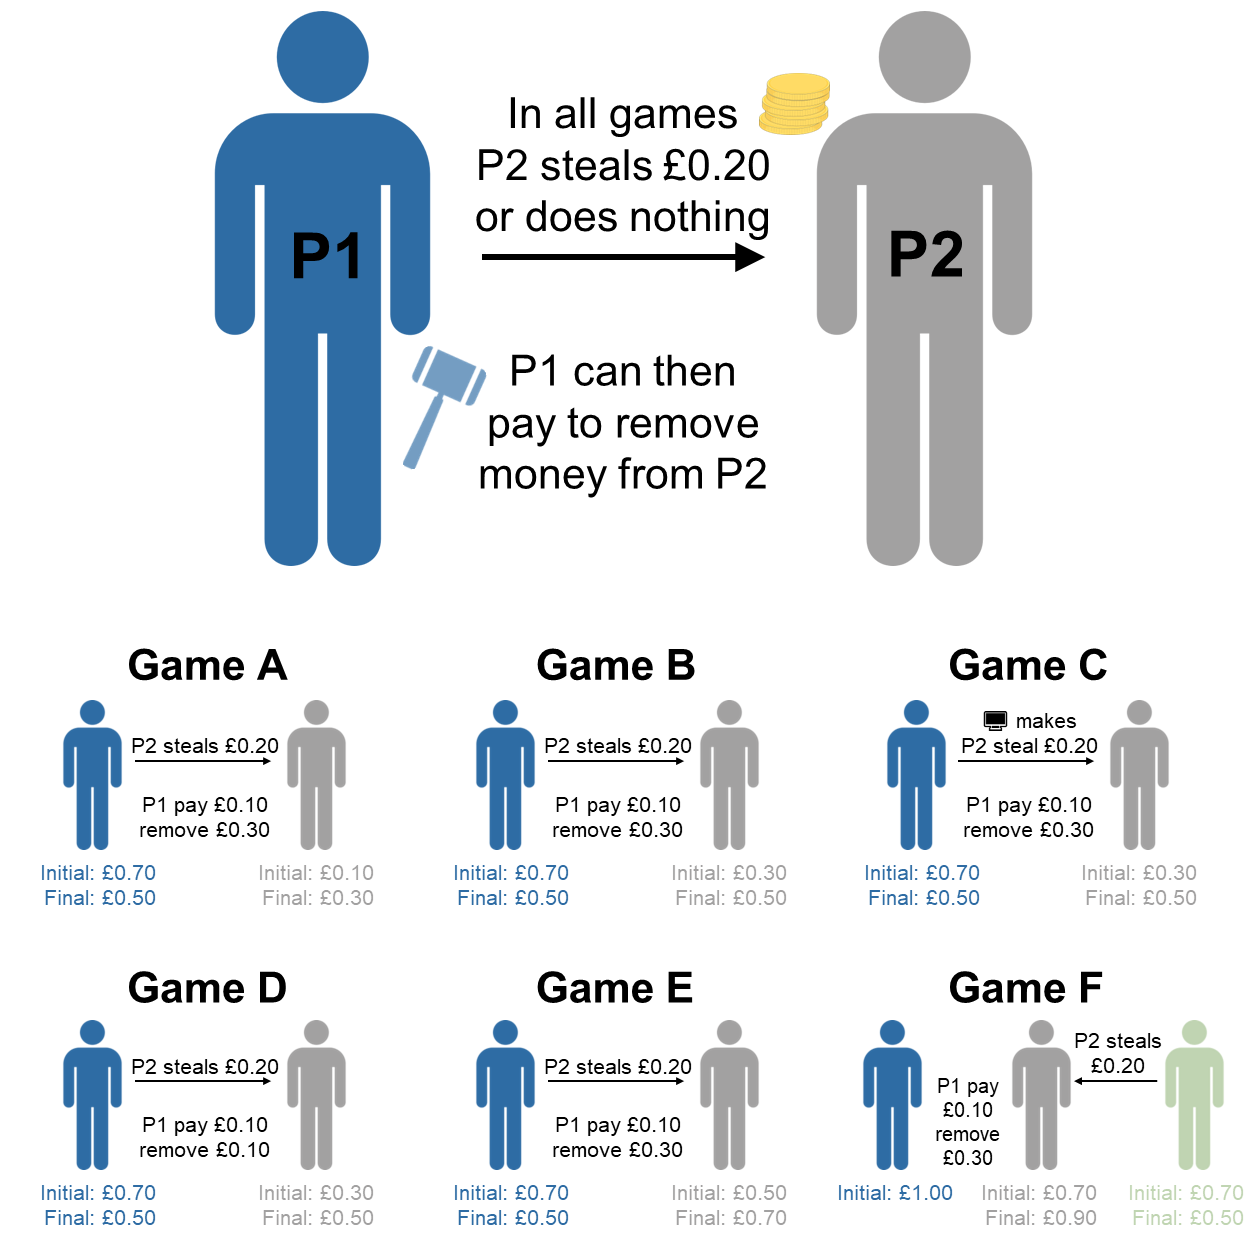
\includegraphics[width=1\linewidth]{images/games} \caption{\emph{Visual summary of the six economic games.} In all
games, Player 2 either steals £0.20 from Player 1 (the focal player) or does
nothing. Player 1 is then given the option to punish by paying a certain amount
of money to remove money from Player 2 (this money is destroyed). The six games
are variants on this general setup, creating situations where (A) Player 2 is
still worse off by stealing, (B) Player 2 creates equality by stealing, (C) the
computer ``decides'' whether Player 2 steals, (D) the fee-fine ratio is 1:1, (E)
Player 2 is better off by stealing, and (F) Player 2 steals instead from a
third-party.}\label{fig:plotGames}
\end{figure}













\begin{lltable}

\scriptsize{

\begin{longtable}{p{1.7cm}p{3.3cm}cccccccccccc}\noalign{\getlongtablewidth\global\LTcapwidth=\longtablewidth}
\caption{\label{tab:tableStrategies}\scriptsize Summary of the different functions for
punishment and the behavioural strategies they predict. \emph{Games A-F are
the games employed in the current study (see Methods for more details). In each
of the six games, participants are given the opportunity to punish players who
``steal'' and those who do not, meaning that participants make twelve punishment
decisions in total. Each behavioural strategy implies a unique pattern of
punishment across all decisions. Green ticks reflect decisions to punish, red
crosses reflect decisions to not punish. In column headers, payoffs at the first
stage (above) and the second stage (below) are denoted as P1-P2 (or P2-P3 {[}P1{]}
for Game F) where participants take the role of P1 and P2 is the target of
punishment. AI = advantageous inequity, DI = disadvantageous inequity.}}\\
\toprule
 &  & \multicolumn{2}{c}{\thead{\scriptsize Game A \\ (AI) \\ 70-10}} & \multicolumn{2}{c}{\thead{\scriptsize Game B \\ (Equal) \\ 70-30}} & \multicolumn{2}{c}{\thead{\scriptsize Game C \\ (Computer) \\ 70-30}} & \multicolumn{2}{c}{\thead{\scriptsize Game D \\ (1:1 Fee-Fine) \\ 70-30}} & \multicolumn{2}{c}{\thead{\scriptsize Game E \\ (DI) \\ 70-50}} & \multicolumn{2}{c}{\thead{\scriptsize Game F \\ (Third-Party) \\ 70-70 [100]}} \\
\cmidrule(r){3-4} \cmidrule(r){5-6} \cmidrule(r){7-8} \cmidrule(r){9-10} \cmidrule(r){11-12} \cmidrule(r){13-14}
Function & \multicolumn{1}{c}{Behavioural strategy} & \multicolumn{1}{c}{\thead{\scriptsize Steal \\ 50-30}} & \multicolumn{1}{c}{\thead{\scriptsize No steal \\ 70-10}} & \multicolumn{1}{c}{\thead{\scriptsize Steal \\ 50-50}} & \multicolumn{1}{c}{\thead{\scriptsize No steal \\ 70-30}} & \multicolumn{1}{c}{\thead{\scriptsize Steal \\ 50-50}} & \multicolumn{1}{c}{\thead{\scriptsize No steal \\ 70-30}} & \multicolumn{1}{c}{\thead{\scriptsize Steal \\ 50-50}} & \multicolumn{1}{c}{\thead{\scriptsize No steal \\ 70-30}} & \multicolumn{1}{c}{\thead{\scriptsize Steal \\ 50-70}} & \multicolumn{1}{c}{\thead{\scriptsize No steal \\ 70-50}} & \multicolumn{1}{c}{\thead{\scriptsize Steal \\ 50-90 [100]}} & \multicolumn{1}{c}{\thead{\scriptsize No steal \\ 70-70 [100]}}\\
\midrule
\endfirsthead
\caption*{\normalfont{Table \ref{tab:tableStrategies} continued}}\\
\toprule
 &  & \multicolumn{2}{c}{\thead{\scriptsize Game A \\ (AI) \\ 70-10}} & \multicolumn{2}{c}{\thead{\scriptsize Game B \\ (Equal) \\ 70-30}} & \multicolumn{2}{c}{\thead{\scriptsize Game C \\ (Computer) \\ 70-30}} & \multicolumn{2}{c}{\thead{\scriptsize Game D \\ (1:1 Fee-Fine) \\ 70-30}} & \multicolumn{2}{c}{\thead{\scriptsize Game E \\ (DI) \\ 70-50}} & \multicolumn{2}{c}{\thead{\scriptsize Game F \\ (Third-Party) \\ 70-70 [100]}} \\
\cmidrule(r){3-4} \cmidrule(r){5-6} \cmidrule(r){7-8} \cmidrule(r){9-10} \cmidrule(r){11-12} \cmidrule(r){13-14}
Function & \multicolumn{1}{c}{Behavioural strategy} & \multicolumn{1}{c}{\thead{\scriptsize Steal \\ 50-30}} & \multicolumn{1}{c}{\thead{\scriptsize No steal \\ 70-10}} & \multicolumn{1}{c}{\thead{\scriptsize Steal \\ 50-50}} & \multicolumn{1}{c}{\thead{\scriptsize No steal \\ 70-30}} & \multicolumn{1}{c}{\thead{\scriptsize Steal \\ 50-50}} & \multicolumn{1}{c}{\thead{\scriptsize No steal \\ 70-30}} & \multicolumn{1}{c}{\thead{\scriptsize Steal \\ 50-50}} & \multicolumn{1}{c}{\thead{\scriptsize No steal \\ 70-30}} & \multicolumn{1}{c}{\thead{\scriptsize Steal \\ 50-70}} & \multicolumn{1}{c}{\thead{\scriptsize No steal \\ 70-50}} & \multicolumn{1}{c}{\thead{\scriptsize Steal \\ 50-90 [100]}} & \multicolumn{1}{c}{\thead{\scriptsize No steal \\ 70-70 [100]}}\\
\midrule
\endhead
Deterrent & Punish to deter another who has harmed you from harming you again in the future & \Large \color{green} \checkmark \normalcolor \scriptsize & \Large \color{red}         x     \normalcolor \scriptsize & \Large \color{green} \checkmark \normalcolor \scriptsize & \Large \color{red}         x     \normalcolor \scriptsize & \Large \color{red}         x     \normalcolor \scriptsize & \Large \color{red}         x     \normalcolor \scriptsize & \Large \color{green} \checkmark \normalcolor \scriptsize & \Large \color{red}         x     \normalcolor \scriptsize & \Large \color{green} \checkmark \normalcolor \scriptsize & \Large \color{red}         x     \normalcolor \scriptsize & \Large \color{red}         x     \normalcolor \scriptsize & \Large \color{red}         x     \normalcolor \scriptsize\\
Norm-enforcing & Punish to enforce a shared anti-harm norm and encourage future norm compliance, even amongst third parties & \Large \color{green} \checkmark \normalcolor \scriptsize & \Large \color{red}         x     \normalcolor \scriptsize & \Large \color{green} \checkmark \normalcolor \scriptsize & \Large \color{red}         x     \normalcolor \scriptsize & \Large \color{red}         x     \normalcolor \scriptsize & \Large \color{red}         x     \normalcolor \scriptsize & \Large \color{green} \checkmark \normalcolor \scriptsize & \Large \color{red}         x     \normalcolor \scriptsize & \Large \color{green} \checkmark \normalcolor \scriptsize & \Large \color{red}         x     \normalcolor \scriptsize & \Large \color{green} \checkmark \normalcolor \scriptsize & \Large \color{red}         x     \normalcolor \scriptsize\\
Retributive & Punish if doing so harms another who has harmed you & \Large \color{green} \checkmark \normalcolor \scriptsize & \Large \color{red}         x     \normalcolor \scriptsize & \Large \color{green} \checkmark \normalcolor \scriptsize & \Large \color{red}         x     \normalcolor \scriptsize & \Large \color{green} \checkmark \normalcolor \scriptsize & \Large \color{red}         x     \normalcolor \scriptsize & \Large \color{green} \checkmark \normalcolor \scriptsize & \Large \color{red}         x     \normalcolor \scriptsize & \Large \color{green} \checkmark \normalcolor \scriptsize & \Large \color{red}         x     \normalcolor \scriptsize & \Large \color{red}         x     \normalcolor \scriptsize & \Large \color{red}         x     \normalcolor \scriptsize\\
Avoid DI & Punish if doing so avoids disadvantageous inequity for self & \Large \color{red}         x     \normalcolor \scriptsize & \Large \color{red}         x     \normalcolor \scriptsize & \Large \color{red}         x     \normalcolor \scriptsize & \Large \color{red}         x     \normalcolor \scriptsize & \Large \color{red}         x     \normalcolor \scriptsize & \Large \color{red}         x     \normalcolor \scriptsize & \Large \color{red}         x     \normalcolor \scriptsize & \Large \color{red}         x     \normalcolor \scriptsize & \Large \color{green} \checkmark \normalcolor \scriptsize & \Large \color{red}         x     \normalcolor \scriptsize & \Large \color{red}         x     \normalcolor \scriptsize & \Large \color{red}         x     \normalcolor \scriptsize\\
Egalitarian & Punish if doing so makes payoffs for all more equal & \Large \color{red}         x     \normalcolor \scriptsize & \Large \color{red}         x     \normalcolor \scriptsize & \Large \color{red}         x     \normalcolor \scriptsize & \Large \color{red}         x     \normalcolor \scriptsize & \Large \color{red}         x     \normalcolor \scriptsize & \Large \color{red}         x     \normalcolor \scriptsize & \Large \color{red}         x     \normalcolor \scriptsize & \Large \color{red}         x     \normalcolor \scriptsize & \Large \color{green} \checkmark \normalcolor \scriptsize & \Large \color{red}         x     \normalcolor \scriptsize & \Large \color{green} \checkmark \normalcolor \scriptsize & \Large \color{red}         x     \normalcolor \scriptsize\\
Seek AI & Punish if doing so produces advantageous inequity for self & \Large \color{red}         x     \normalcolor \scriptsize & \Large \color{red}         x     \normalcolor \scriptsize & \Large \color{green} \checkmark \normalcolor \scriptsize & \Large \color{red}         x     \normalcolor \scriptsize & \Large \color{green} \checkmark \normalcolor \scriptsize & \Large \color{red}         x     \normalcolor \scriptsize & \Large \color{red}         x     \normalcolor \scriptsize & \Large \color{red}         x     \normalcolor \scriptsize & \Large \color{red}         x     \normalcolor \scriptsize & \Large \color{red}         x     \normalcolor \scriptsize & \Large \color{red}         x     \normalcolor \scriptsize & \Large \color{red}         x     \normalcolor \scriptsize\\
Competitive & Punish if doing so improves your relative position & \Large \color{green} \checkmark \normalcolor \scriptsize & \Large \color{green} \checkmark \normalcolor \scriptsize & \Large \color{green} \checkmark \normalcolor \scriptsize & \Large \color{green} \checkmark \normalcolor \scriptsize & \Large \color{green} \checkmark \normalcolor \scriptsize & \Large \color{green} \checkmark \normalcolor \scriptsize & \Large \color{red}         x     \normalcolor \scriptsize & \Large \color{red}         x     \normalcolor \scriptsize & \Large \color{green} \checkmark \normalcolor \scriptsize & \Large \color{green} \checkmark \normalcolor \scriptsize & \Large \color{green} \checkmark \normalcolor \scriptsize & \Large \color{green} \checkmark \normalcolor \scriptsize\\
Antisocial & Punish exclusively those who do not cause harm & \Large \color{red}         x     \normalcolor \scriptsize & \Large \color{green} \checkmark \normalcolor \scriptsize & \Large \color{red}         x     \normalcolor \scriptsize & \Large \color{green} \checkmark \normalcolor \scriptsize & \Large \color{red}         x     \normalcolor \scriptsize & \Large \color{green} \checkmark \normalcolor \scriptsize & \Large \color{red}         x     \normalcolor \scriptsize & \Large \color{green} \checkmark \normalcolor \scriptsize & \Large \color{red}         x     \normalcolor \scriptsize & \Large \color{green} \checkmark \normalcolor \scriptsize & \Large \color{red}         x     \normalcolor \scriptsize & \Large \color{green} \checkmark \normalcolor \scriptsize\\
Never punish & Never punish others & \Large \color{red}         x     \normalcolor \scriptsize & \Large \color{red}         x     \normalcolor \scriptsize & \Large \color{red}         x     \normalcolor \scriptsize & \Large \color{red}         x     \normalcolor \scriptsize & \Large \color{red}         x     \normalcolor \scriptsize & \Large \color{red}         x     \normalcolor \scriptsize & \Large \color{red}         x     \normalcolor \scriptsize & \Large \color{red}         x     \normalcolor \scriptsize & \Large \color{red}         x     \normalcolor \scriptsize & \Large \color{red}         x     \normalcolor \scriptsize & \Large \color{red}         x     \normalcolor \scriptsize & \Large \color{red}         x     \normalcolor \scriptsize\\
\bottomrule
\end{longtable}

}

\end{lltable}

\hypertarget{results}{%
\section{Results}\label{results}}

The overall pattern of punitive behaviour in the six economic games was in line
with previous research and very similar across both countries (Figure
\ref{fig:plotDecisions}). Participants were generally more likely to punish
targets who stole from another individual compared to targets who did not steal
(multilevel logistic regression; \emph{b} =
1.93, standard error =
0.27, \emph{p}
\textless{} .001). Participants were also more likely
to punish when targets' stealing behaviour generated inequalities,
specifically in Games E and F (\emph{b} =
2.42, SE = 0.44,
\emph{p} \textless{} .001).





\begin{figure}
\centering
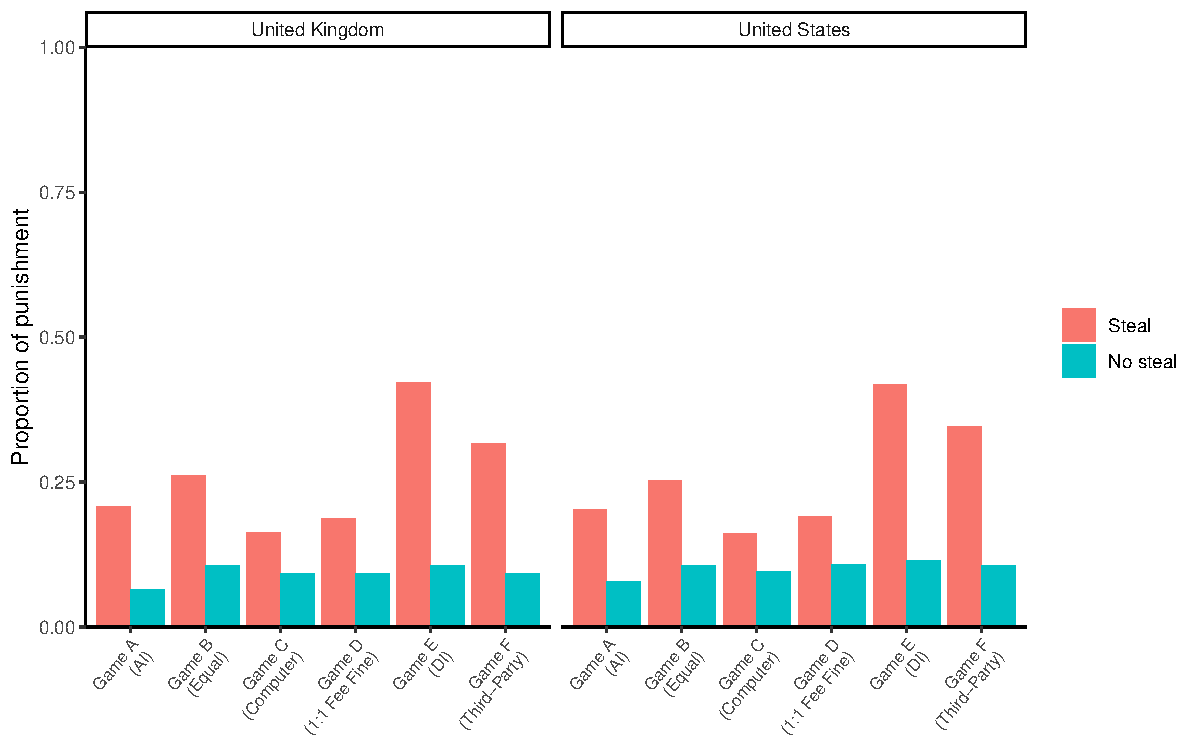
\includegraphics{manuscript_files/figure-latex/plotDecisions-1.pdf}
\caption{\label{fig:plotDecisions}\emph{Overall pattern of punitive behaviour across all six
economic games, split by country.} AI = advantageous inequity, DI =
disadvantageous inequity.}
\end{figure}

We classified participants into a particular strategy if their behaviour across
all twelve decisions matched our behavioural predictions shown in Table
\ref{tab:tableStrategies} exactly. Table \ref{tab:tableStrategyCounts} shows
the proportion of participants following each strategy, with N/A used to
represent participants who did not fit exactly into any particular strategy type.
Overall, 59\%
of our participants could be classified exactly into one of the strategies. The
most common strategy in both countries was to never punish across any of the
games. The next most common strategies were those that care about
minimising payoff differences (avoid disadvantageous inequity, egalitarian).
Less common were the behaviour-shaping strategies (deterrent, norm-enforcing),
the retributive strategy, and the competitive strategies (seek AI, competitive).
Although participants often punished targets who did not steal
in the six games (Figure \ref{fig:plotDecisions}), no participants followed the
antisocial strategy by exclusively punishing targets who did not steal across
\emph{all} games.






\begin{table}[tbp]

\begin{center}
\begin{threeparttable}

\caption{\label{tab:tableStrategyCounts}Counts and proportions of participants
following each punishment strategy exactly, split by country. N/A implies that
participants were unable to be classified exactly into any of the punishment
strategies.}

\begin{tabular}{lcccc}
\toprule
 & \multicolumn{2}{c}{\thead{United Kingdom \\ (N = 1014)}} & \multicolumn{2}{c}{\thead{United States \\ (N = 996)}} \\
\cmidrule(r){2-3} \cmidrule(r){4-5}
Strategy & \multicolumn{1}{c}{N} & \multicolumn{1}{c}{Prop} & \multicolumn{1}{c}{N} & \multicolumn{1}{c}{Prop}\\
\midrule
Deterrent & 9 & 0.009 & 6 & 0.006\\
Norm-enforcing & 8 & 0.008 & 16 & 0.016\\
Retributive & 6 & 0.006 & 5 & 0.005\\
Avoid DI & 67 & 0.066 & 62 & 0.062\\
Egalitarian & 65 & 0.064 & 71 & 0.071\\
Seek AI & 2 & 0.002 & 0 & 0.000\\
Competitive & 3 & 0.003 & 1 & 0.001\\
Antisocial & 0 & 0.000 & 0 & 0.000\\
Never punish & 426 & 0.420 & 447 & 0.449\\
N/A & 428 & 0.422 & 388 & 0.390\\
\bottomrule
\end{tabular}

\end{threeparttable}
\end{center}

\end{table}

To further investigate the strategies that participants were following, we
examined the most common patterns of punitive behaviour across all twelve
decisions. Supplementary Table \ref{tab:tablePatterns} shows the proportion of
participants following the 25 most common behavioural patterns, including,
where appropriate, the predetermined strategies from Table
\ref{tab:tableStrategies}. In both countries, a common pattern of behaviour
not captured by any of the strategies was punishing only when the target stole
in the third-party game (Game F). Punishment in this game is consistent with an
egalitarian motive, as stealing produces unequal outcomes, but third-party
punishment here is also consistent with norm-enforcing and competitive motives
(see Table \ref{tab:tableStrategies}). Other common behavioural patterns not
captured by our strategies included punishing whenever the target stole across
all games and always punishing in every game irrespective of the targets'
behaviour.

While it is useful to look at exact patterns of behaviour, participants may not
have implemented their chosen punishment strategy with exact precision.
In reality, strategies may have been implemented probabilistically for each
punishment decision. There is also the possibility of implementation errors,
whereby participants occasionally ``slip up'' and make decisions that are
incongruent with a particular strategy. This may explain why some participants
were unable to be classified exactly into a single punishment strategy.

To deal with this complexity and include all observed data in our frequency
estimates, we fitted a Bayesian latent state model to the data. This model
assumes that the nine strategies in Table \ref{tab:tableStrategies} (plus a
``random choice'' strategy that chooses randomly for each decision) are the only
latent strategies and that these are instantiated into observed behaviour
according to the logic in Table \ref{tab:tableStrategies} with some
probability of implementation error (i.e., an intention to punish is implemented
as non-punishment and vice versa). Averaging over all strategies and
incorporating the possibility of implementation errors, the model estimates the
probability of participants following any particular strategy, given the
observed data.

The posterior estimates from the model are presented in Figure
\ref{fig:plotModel1b}. The posterior probabilities for each strategy did not
differ between the two countries. In both countries, the never punish strategy
had the highest probability, followed by the egalitarian strategy. The
norm-enforcing and seek AI strategies were the next most likely, with higher
posterior estimates than the competitive and antisocial strategies. None of the
other strategies differed in their posterior estimates. The same general pattern
emerged when we analysed the full dataset without pre-registered exclusions
(Supplementary Figure \ref{fig:plotModel1a}).






\begin{figure}
\centering
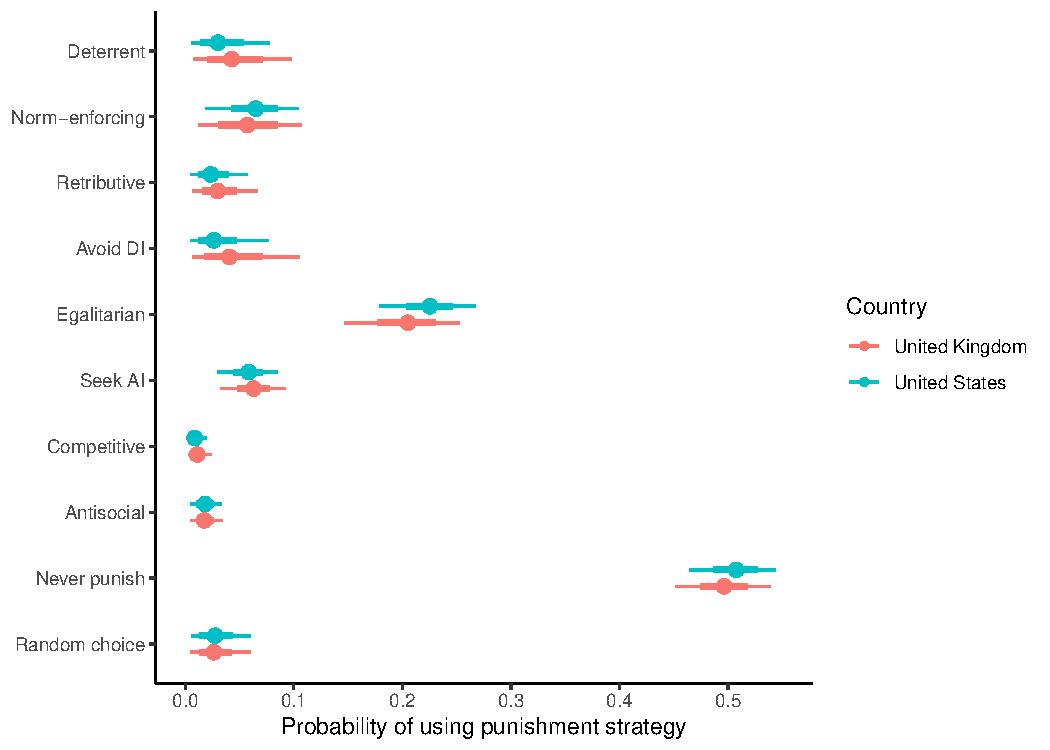
\includegraphics{manuscript_files/figure-latex/plotModel1b-1.pdf}
\caption{\label{fig:plotModel1b}\emph{Posterior estimates of the probabilities of following
different punishment strategies from the Bayesian latent state model.} The model
assumes an implementation error rate of 5\%. Points represent posterior medians,
line ranges represent 50\% and 95\% credible intervals.}
\end{figure}

Next, we explored which traits predicted adherence to different punishment
strategies. To answer this question, we included variables capturing
demographics, personality, social preferences, political views, and religious
views as predictors in our Bayesian latent state model. We included each
variable in a separate model, predicting all ten punishment strategies
(the nine from Table 1, plus the `random choice' strategy) simultaneously.

Demographic variables tended to be unrelated to strategy usage: age and gender
did not predict adherence to a particular punishment strategy (Supplementary
Figures \ref{fig:plotAllDems2} and \ref{fig:plotAllDems1}). In the United
States, the never punish strategy was slightly more common among participants
lower in socio-economic status (median posterior slope =
-0.20, 95\% CI {[}-0.38
-0.02{]}) but this effect was small.

Conversely, personality and social preferences were linked to variation in
punishment strategies. When including the Big-6 personality dimensions and
Social Value Orientation (SVO) in the model, we found associations with the
egalitarian, never punish, and random choice strategies (Figure
\ref{fig:plotAllPers2}). Participants higher in SVO were more likely to follow
the egalitarian and the never punish strategies, while those with lower SVO
scores were more likely to enact the random choice strategy. The personality
dimensions of honesty-humility and openness to experience were both positively
associated with following the never punish strategy, while extraversion
negatively predicted this strategy. The effects were mostly similar across
countries, but occasionally differed: for example, in the United States,
but not in the United Kingdom, honesty-humility was positively associated with
following the egalitarian strategy and negatively associated with following
the random choice strategy. Overall, the same pattern of results emerged when
analysing the full dataset without exclusions (Supplementary Figure
\ref{fig:plotAllPers1}).







\begin{figure}
\centering
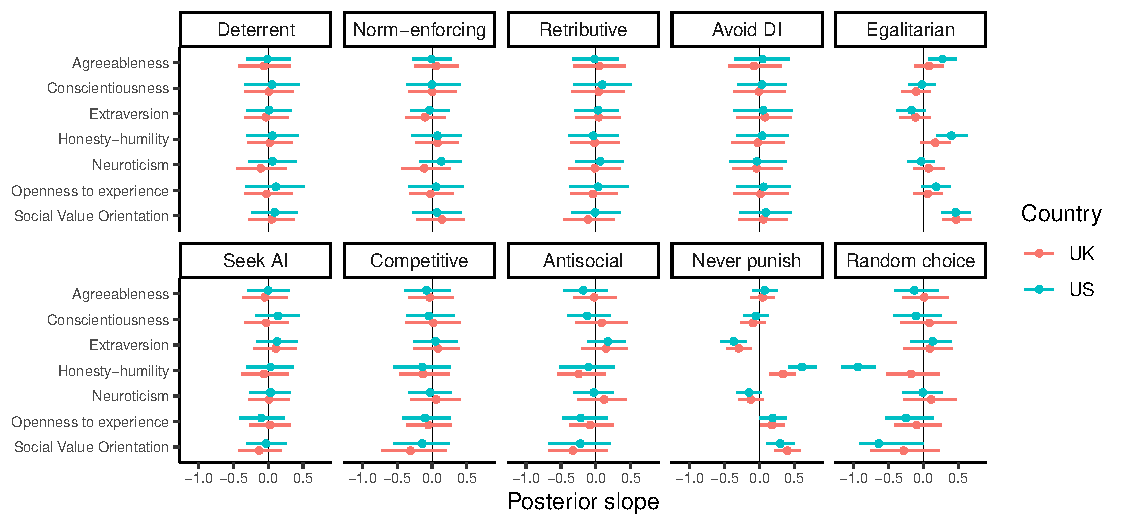
\includegraphics{manuscript_files/figure-latex/plotAllPers2-1.pdf}
\caption{\label{fig:plotAllPers2}\emph{Posterior slopes from Bayesian latent state models
including Big-6 personality dimensions and Social Value Orientation.} Each row
represents a separate model. All models assume an implementation error rate of
5\%. Points represent posterior medians, line ranges represent 95\% credible
intervals.}
\end{figure}

Political and religious variables were also associated with punishment strategy
(Figure \ref{fig:plotAllPolRel2}). These effects tended to be more pronounced
in the United States. Controlling for Social Dominance Orientation, American
participants higher in Right Wing Authoritarianism were more likely to follow
the strategies avoiding disadvantageous inequity and seeking advantageous
inequity. Participants who stated that they would like to ``bring those below
them {[}on the socio-economic status ladder{]} up a peg'' were more likely to follow
the egalitarian strategy, while American participants higher in Social Dominance
Orientation, Right Wing Authoritarianism, and believing that God controls events
in the world were less likely to follow the egalitarian strategy. In general,
religious and conservative participants were less likely to follow the never
punish strategy. This general pattern of results was replicated with the full
dataset (Supplementary Figure \ref{fig:plotAllPolRel1}).








\begin{figure}
\centering
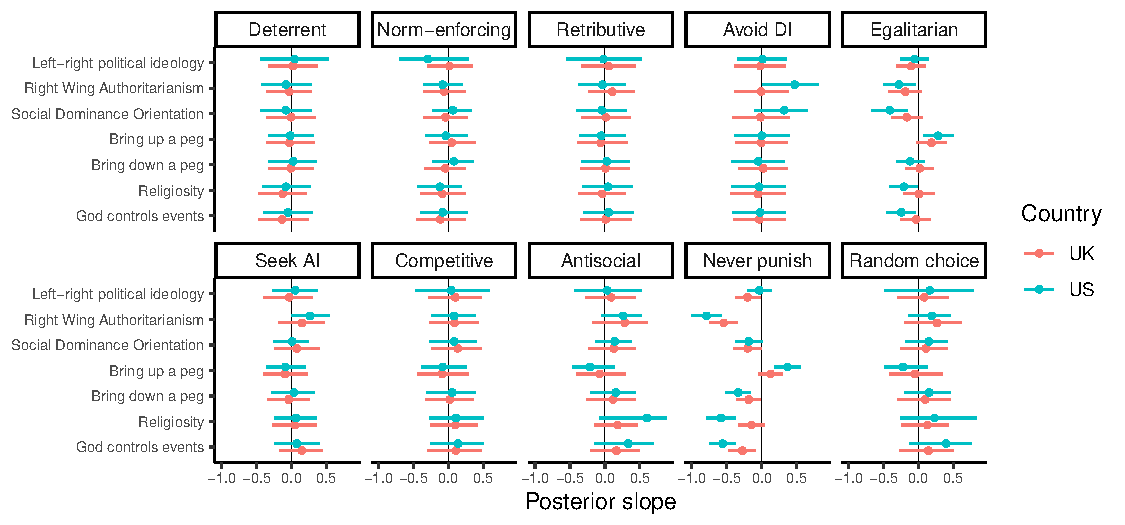
\includegraphics{manuscript_files/figure-latex/plotAllPolRel2-1.pdf}
\caption{\label{fig:plotAllPolRel2}\emph{Posterior slopes from Bayesian latent state models
including political ideology, views about social inequality, and religiosity.}
Each row represents a separate model aside from Social Dominance Orientation and
Right Wing Authoritarianism, which control for one another within the same
model. All models assume an implementation error rate of 5\%. Points represent
posterior medians, line ranges represent 95\% credible intervals.}
\end{figure}

Finally, we asked whether participants had insight into their own punishment
strategy. In other words, could participants self-report the strategy that they
were following during the games? To answer this question, we included
participants' responses to post-game questions about their strategy as
predictors in the model. As before, each predictor was included in a separate
model, predicting all ten strategies simultaneously.

In general, we found that self-reported strategy usage was positively associated
with the behavioural strategy that participants employed (see Supplementary
Figures \ref{fig:plotSliders1} and \ref{fig:plotSliders2} for the distribution
of responses to self-report questions). Figure \ref{fig:plotAllSliders2} shows
the relationships between self-report questions and the different punishment
strategies, highlighting the combinations where the question matched the
behavioural strategy. We found positive relationships between the self-report
questions and strategy usage for the norm-enforcing, egalitarian, seek
advantageous inequity, never punish, and random choice strategies. The 95\%
credible intervals for other estimates included zero, though these estimates
often trended in a positive direction. The same pattern of results was found
when analysing the full dataset without exclusions (Supplementary Figure
\ref{fig:plotAllSliders1}).








\begin{figure}
\centering
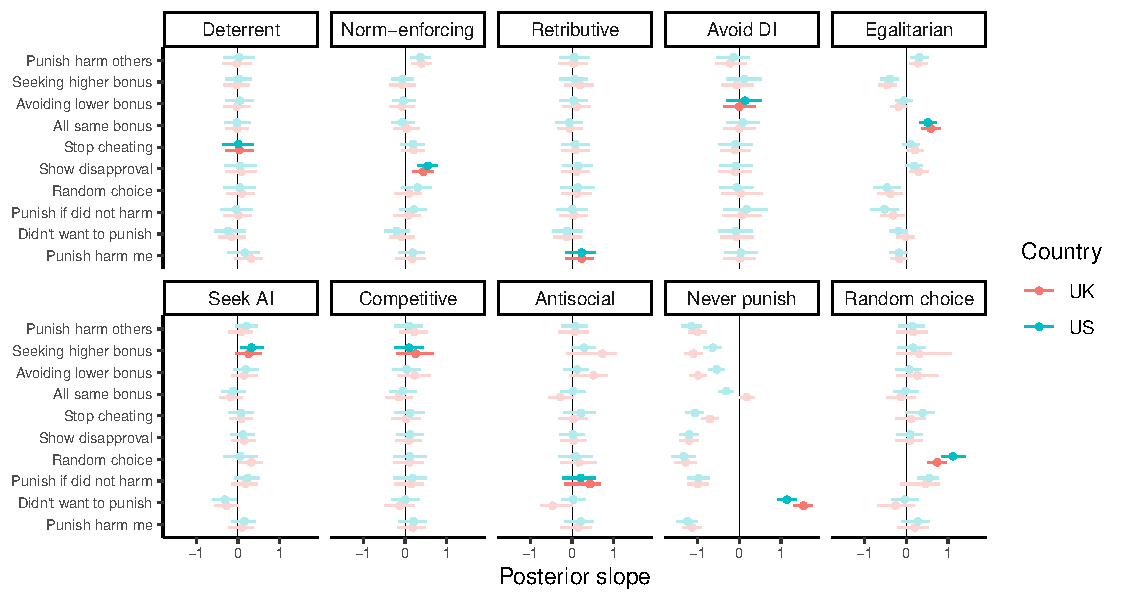
\includegraphics{manuscript_files/figure-latex/plotAllSliders2-1.pdf}
\caption{\label{fig:plotAllSliders2}\emph{Posterior slopes from models including
self-reported strategy usage.} Each row represents a separate model. All models
assume an implementation error rate of 5\%. Highlighted estimates represent
combinations where the self-report question matched the behavioural strategy.
Points represent posterior medians, line ranges represent 95\% credible
intervals.}
\end{figure}

\hypertarget{discussion}{%
\section{Discussion}\label{discussion}}

Using a suite of economic games measuring punishment in different situations,
we have shown that punishment does not serve just one function, but instead is
a flexible tool that can be and is used for different purposes\textsuperscript{15}.
Punishment is more akin to a swiss army knife than a hammer, used by some to
enforce norms of cooperation and by others to reduce or even create inequality
between individuals. We found that people's punishment strategy can, to some
extent, be predicted by individual differences in personality, social
preferences, and political and religious views. Moreover, contrary to the view
that people are often unable to articulate the reasons for their punitive
behaviour\textsuperscript{28}, people seem to have some degree of insight into the
strategy they are using. Despite small differences, these general patterns
replicated in samples from both the United Kingdom and the United States.

Among the punitive strategies, the most common were particularly sensitive to
inequality in payoffs, either from a self-referential perspective (i.e., avoid
disadvantageous inequity) or more generally (i.e., egalitarian). This is in
line with previous studies which have highlighted inequity aversion as an
important motivation for punishment in economic games\textsuperscript{29,30}. Personality and social preference variables mapped
onto these strategies in expected ways. Traits associated with other-regarding
concern, such as SVO and honesty-humility, predicted following the egalitarian
strategy, whereas religious and conservative individuals were less likely to
follow this strategy, especially in the United States. Moreover, participants
following the egalitarian strategy were able to self-report this strategy,
though the same was not true for the avoid disadvantageous inequity strategy.

Behaviour shaping strategies, such as deterrence and norm-enforcement, were less
common than strategies sensitive to inequality in our set of games. This was
reflected both in participants' elicited punishment behaviour (Figure
\ref{fig:plotModel1b}) and in their self-reports of their own strategy
(Supplementary Figures \ref{fig:plotSliders1} and \ref{fig:plotSliders2}).
Regarding the predictors of these strategies, we found that demographic,
personality, political, and religious variables tended to be unrelated to
deterrent and norm-enforcing punishment strategies. We also found that
participants had insight into the norm-enforcing strategy, but not the deterrent
strategy. This finding is in line with previous research showing that people
struggle to accurately report the deterrent motivations for their punitive
behaviour\textsuperscript{28}.

Other punitive strategies were less common in our dataset, but some were more
prevalent than others. For example, participants were more likely to use
punishment to seek advantageous inequity than to exclusively harm those who did
not steal (i.e., antisocial punishment). The existence of the ``seek AI'' strategy
in our dataset supports the claim that punishment can also be used as a tool to
increase one's own relative position\textsuperscript{15}. While generally rare, we
found that this motive for punishment was more common among authoritarian
participants, at least in the United States, potentially providing an
explanation for why peer punishment has been found to be more common among
conservatives in previous work\textsuperscript{41}. Moreover, the fact that no
participants in our sample punished non-stealing across all games suggests that
antisocial punishment does not function to harm cooperators specifically, as has
been previously suggested\textsuperscript{17}. Instead, antisocial punishment appears
to be motivated by improving one's relative position in general, which is in
line with work showing that antisocial punishment disappears with a 1:1 fee-fine
ratio\textsuperscript{35}.

The fact that people use punishment for many different reasons poses problems
for the way that punishment is operationalised in classic behavioural economic
game studies. In these studies, a common assumption is that participants will
punish to change the behaviour of cheats. But in reality, people may be choosing
the punishment option to achieve a variety of different goals. The targets of
punishment in these studies are likely well aware that punishment could be
levied for these different reasons and this knowledge may impact their
responses. For example, if cheating targets interpret punishment as serving a
competitive motive, it may elicit retaliation rather than encourage
cooperation\textsuperscript{9,15,50}. This might help to
explain the mixed findings in the field as to whether punishment actually
motivates cheating targets to cooperate in the future\textsuperscript{15}.

It is striking that the most common strategy in our dataset was to never punish.
This is partly because punishment in these games imposes an economic cost for no
tangible benefit. If the fee-fine ratio had been lower such that it was cheaper
to punish, we may have seen more punishment from participants. Indeed,
72\%
of participants following the never punish strategy positively stated that they
didn't want to pay to reduce anyone's bonus but would have done so if it were
free. But the frequency of the never punish strategy perhaps also reflects a
more general aversion to peer punishment, an aversion that has been highlighted
in both WEIRD (Western, educated, industrialised, rich, and democratic) samples\textsuperscript{51,52} and in small-scale societies\textsuperscript{53}.
One reason that people may be averse to peer punishment is that, due to its
multipurpose nature, it may be interpreted as a competitive challenge by targets
and trigger retaliation\textsuperscript{15}. In situations that lack clear
institutional norms to legitimise punishment, such as our economic games and
some situations in the real world, people might abstain from peer punishment to
avoid such retaliation, regardless of whether retaliation is actually possible.
By contrast, institutionalised punishment in small-scale societies often
functions to compensate victims adequately while limiting the potential for
feuds and cycles of retaliation\textsuperscript{54,55}. Future research
should uncover whether people are more willing to punish in these
conventionalised contexts.

There are several limitations with our study design that can guide future
research. First, we used one-shot economic games to measure punishment
strategies, which may have led us to underestimate behaviour-change strategies
like deterrence. Our inclusion of Game C somewhat mitigated this issue by
manipulating whether stealing behaviour was intentional vs.~unintentional and
thus whether there was any behaviour to be deterred. Due to limits on our
within-subjects design and the complexity of the strategy space, it was not
feasible for us to expand our study to include additional contexts to elicit
behaviour-change strategies (e.g., repeated games, games where targets are not
made aware of the punishment, games where targets can retaliate). Future work
could study these contexts separately.

A second limitation is that some strategies required more punishment than others
to be met. For example, the competitive strategy required punishment in ten of
twelve decisions, compared to the avoid disadvantageous inequity strategy which
required only one instance of punishment (Table \ref{tab:tableStrategies}).
Strategies thus differed in how ``expensive'' they were to implement, perhaps
explaining why some strategies were more common than others. This issue is
largely unavoidable in our design since strategies, by their very nature, differ
in how punitive they are. To partially mitigate this issue, we employed the
strategy method to incentivise participants, such that payoffs were calculated
from a randomly chosen game instead of summed across all games.

Another limitation is that our results may be contingent on the particular suite
of anonymous stealing games that we used. With our anonymous design, we were
unable to study other potential reputational strategies underlying punishment,
such as signalling trustworthiness\textsuperscript{47}. Moreover, stealing may be
evaluated differently to other forms of cheating, such as not contributing to
public goods, and other negative behaviours, such as lying or breaking taboos.
Finally, we were unable to include all permutations of situational features in
the games (e.g., second-party vs.~third-party, equal vs.~unequal) making it
difficult to interpret some patterns of behaviour. For example, many
participants punished only in the third-party game (Game F), but it is not clear
whether these participants were driven by the third-party nature of the game or
simply by the fact that stealing in that game generated inequality. Future work
should determine whether different reputational contexts, target behaviours, and
combinations of situational features elicit different punishment strategies.

In sum, we have shown that while many people choose not to punish peers, those
who do are motivated by a variety of different concerns, including behaviour
shaping, egalitarianism, and competition. Much like the observed variation in
human social learning strategies\textsuperscript{39}, humans thus also exhibit
variation in their punishment strategies. These individual differences map onto
personality dimensions, social preferences, political and religious views, and
self-reports of behaviour. We hope that future work will continue to unpack the
multifaceted nature of human punishment.

\hypertarget{methods}{%
\section{Methods}\label{methods}}

\hypertarget{ethical-approval}{%
\subsection{Ethical approval}\label{ethical-approval}}

Ethical approval was granted by the University College London Ethics Board
(project: 3720/002). The study was performed in accordance with all the relevant
guidelines and regulations. Informed consent was obtained from all participants
prior to the study.

\hypertarget{pre-registration}{%
\subsection{Pre-registration}\label{pre-registration}}

We pre-registered the study on the Open Science Framework before collecting data
in the United Kingdom (11\textsuperscript{th} November 2022; \url{https://osf.io/k75fc}). We submitted
another pre-registration before collecting data in the United States (20\textsuperscript{th}
June 2023; \url{https://osf.io/q4hdy}). In the pre-registrations, we outlined our
study design, exclusion criteria, and analysis plan. As the study was
exploratory, we did not pre-register any explicit hypotheses. We did not deviate
from the pre-registrations.

\hypertarget{exclusion-criteria}{%
\subsection{Exclusion criteria}\label{exclusion-criteria}}

We pre-registered that we would exclude participants who failed any of the
attention checks, sped through the surveys (i.e., two standard deviations below
the median duration), or flatlined (i.e., provided identical responses to matrix
questions). We also stated that we would exclude data for particular games if
participants failed the comprehension question for that game. We followed our
pre-registered plan of conducting analyses with and without these exclusions
(analyses without exclusions are reported in the Supplementary Material).

\hypertarget{participants}{%
\subsection{Participants}\label{participants}}

We collected a representative sample of 1019 participants
from the United Kingdom through the online platform Prolific
(\url{https://www.prolific.com/}). All of these participants completed the economic
games and 973 returned to complete the follow-up survey a
week later (95\% retention
rate). After exclusions, we were left with 1014 participants
overall (see Supplementary Figure \ref{fig:plotSampleUK} for sample
characteristics).

We later collected a representative sample of 1005
participants from the United States through Prolific. All of these participants
completed the economic games and 957 returned to complete
the follow-up survey (95\%
retention rate). After exclusions, we were left with 996
participants overall (see Supplementary Figure \ref{fig:plotSampleUS} for
sample characteristics).

\hypertarget{materials}{%
\subsection{Materials}\label{materials}}

\hypertarget{economic-games}{%
\subsubsection{Economic games}\label{economic-games}}

In the first part of the study, participants completed six economic games, each
with slight variations. In all games, there are multiple players and the
participant takes the role of P1. P2 either (a) steals £0.20 from another player
and adds it to their payoff or (b) does nothing. For each of these cases,
participants are asked whether they would like to pay money to reduce P2's
payoff. Games A-E have two players and Game F has three players.

The six games are as follows (variations bolded; see Figure \ref{fig:plotGames}
for a visual representation of the games):

\begin{enumerate}
\def\labelenumi{\arabic{enumi}.}
\tightlist
\item
  \emph{Game A (Advantageous Inequity)}. P1 starts with £0.70 and P2 starts with
  £0.10. P2 is given the option to either steal £0.20 from P1 or do nothing. P1
  can then pay £0.10 to reduce P2's payoff by £0.30.
\item
  \emph{Game B (Equal)}. P1 starts with £0.70 and P2 starts with \textbf{£0.30}. P2 is
  given the option to either steal £0.20 from P1 or do nothing. P1 can then pay
  £0.10 to reduce P2's payoff by £0.30.
\item
  \emph{Game C (Computer)}. P1 starts with £0.70 and P2 starts with £0.30.
  Participants are told that \textbf{``the computer will decide''} whether P2 steals
  £0.20 from P1 or does nothing. P1 can then pay £0.10 to reduce P2's payoff by
  £0.30.
\item
  \emph{Game D (1:1 Fee-Fine)}. P1 starts with £0.70 and P2 starts with £0.30. P2 is
  given the option to either steal £0.20 from P1 or do nothing. P1 can then pay
  £0.10 to reduce P2's payoff by \textbf{£0.10}.
\item
  \emph{Game E (Disadvantageous Inequity)}. P1 starts with £0.70 and P2 starts with
  \textbf{£0.50}. P2 is given the option to either steal £0.20 from P1 or do
  nothing. P1 can then pay £0.10 to reduce P2's payoff by £0.30.
\item
  \emph{Game F (Third-Party)}. P1 starts with £1.00, P2 and P3 start with £0.70. P2
  is given the option to either steal £0.20 \textbf{from P3} or do nothing. P1 can
  then pay £0.10 to reduce P2's payoff by £0.30.
\end{enumerate}

For each game, participants saw the game instructions and answered a
comprehension question before providing their decisions. After completing all
the games, participants were asked to give an open-ended response explaining
their behaviour in the games, and then responded to several slider questions
capturing the different reasons for their decisions (for full wordings, see
Supplementary Table \ref{tab:tableSliderWordings}).

\hypertarget{survey-questions}{%
\subsubsection{Survey questions}\label{survey-questions}}

In a follow-up survey, we collected the following data on participants (for
wordings of all questions, see Supplementary Table
\ref{tab:tableSurveyWordings}):

\begin{itemize}
\tightlist
\item
  \emph{Demographics}. In the survey, we collected information on participants'
  education level and self-reported socio-economic status (MacArthur ladder\textsuperscript{56}). We also collected additional demographic data from Prolific
  (e.g., age, gender, student status).
\item
  \emph{Personality}. We used the Mini-IPIP scale\textsuperscript{57} to measure the Big 6
  personality dimensions of agreeableness, conscientiousness, extraversion,
  honesty-humility, openness to experience, and neuroticism (four items each).
\item
  \emph{Social Value Orientation}. We used the Social Value Orientation Slider
  Measure to measure other-regarding preferences\textsuperscript{58}. Across fifteen
  items, participants made decisions on how to allocate different amounts of
  money between themselves and another anonymous individual. From these
  decisions, we calculated participants' Social Value Orientation ``angle'' as a
  measure of their other-regarding preference, following the steps outlined in
  ref\textsuperscript{58}.
\item
  \emph{Political ideology}. We included several measures of political ideology,
  including left-right conservatism, Social Dominance Orientation\textsuperscript{59}
  (eight items), and Right Wing Authoritarianism\textsuperscript{60} (six items).
  We also probed participants' views on social inequality by asking them whether
  they would like to bring people above (below) them on the MacArthur
  socio-economic status ladder down (up) a peg or two.
\item
  \emph{Religious views}. We asked participants how religious they consider
  themselves and whether they believe that God or another spiritual non-human
  entity controls the events in the world\textsuperscript{61}.
\end{itemize}

\hypertarget{procedure}{%
\subsection{Procedure}\label{procedure}}

We began data collection in the United Kingdom on 28\textsuperscript{th} November 2022, with
participants returning to complete the follow-up survey on 5\textsuperscript{th} December 2022.
We then ran a second wave of data collection in the United States on 20\textsuperscript{th} June
2023, with participants returning to complete the follow-up survey on 27\textsuperscript{th}
June 2023. Our surveys were designed through the online survey platform
Qualtrics (\url{https://www.qualtrics.com/}).

In the initial games survey, participants completed all six economic games in a
random order, with punishment decisions (whether to punish a stealing target and
whether to punish a target who did nothing) randomised within games. Responses
to comprehension questions suggested that participants understood the six
economic games (Supplementary Table \ref{tab:tableComp}). We used the strategy
method to incentivise the economic games, choosing a random game to determine
bonus payment. After all games,
62\%
of participants stated that they believed that their decisions had real
consequences for others.

In the follow-up survey, participants completed blocks of questions on
demographics, personality, Social Value Orientation, political ideology, and
religious views in a random order, with questions randomised within blocks. A
random decision from the Social Value Orientation Slider Measure was chosen to
determine bonus payment.

Participants were paid £1.80 for completing the games survey, plus a bonus
payment from the six economic games (between £0.40 -- £0.70 depending on their
decision). Participants were paid £1.50 for completing the follow-up survey,
plus a bonus payment from the Social Value Orientation Slider Measure (between
£0.50 -- £0.85 depending on their decision).

\hypertarget{statistical-analysis}{%
\subsection{Statistical analysis}\label{statistical-analysis}}

We pre-registered that we would use a Bayesian latent state model to infer
unobserved punishment strategies from the observed data (for a similar version
of this model, see ref\textsuperscript{62}). In this model, participants \(i\) in
countries \(c\) make binary punishment decisions across twelve decisions \(j\). We
assume that the probability of the observed data \(y_{i,j}\) is the weighted
average of the probability of the observed data conditional on each of the ten
punishment strategies \(s\). From this logic, the model estimates the probability
of each strategy \(p_{s}\). The full model is as follows:

\begin{align}
y_{i,j} &\sim \text{Bernoulli}(\theta_{j}) \\
\theta_{j} &= \sum_{s=1}^{10} p_{s} \text{Pr}(\text{punish}|s,j) \nonumber \\
p &= \text{softmax}(\alpha_{c[i]}) \nonumber \\
\alpha_{s,c} &\sim \text{Normal(0, 1)} \nonumber
\end{align}

The conditional probabilities \(\text{Pr}(\text{punish}|s,j)\) are hard coded in
the model as outlined in Table \ref{tab:tableStrategies}. We incorporate an
implementation error rate \(\delta\) into these conditional probabilities by coding
green ticks in Table \ref{tab:tableStrategies} with a conditional probability
of \(1 - \delta\) and coding red crosses with a conditional probability of
\(0 + \delta\). The random choice is consistently coded with a conditional
probability of ½ across all decisions.

To include a categorical predictor in the model, we estimate a different
\(\alpha_{s,c}\) for each categorical level. To include a continuous predictor
\(x\) in the model, we include a slope \(\beta\) in the linear model for \(p\):

\begin{align}
y_{i,j} &\sim \text{Bernoulli}(\theta_{j}) \\
\theta_{j} &= \sum_{s=1}^{10} p_{s} \text{Pr}(\text{punish}|s,j) \nonumber \\
p &= \text{softmax}(\alpha_{c[i]} + \beta_{c[i]}x_{i}) \nonumber \\
\alpha_{s,c} &\sim \text{Normal(0, 1)} \nonumber \\
\beta_{s,c} &\sim \text{Normal(0, 0.2)} \nonumber
\end{align}

We estimated the posterior distributions of these models using Hamiltonian Monte
Carlo as implemented in Stan version 2.26.1\textsuperscript{63}. We ran each model for
2000 samples, with 1000 warmup samples. R-hat values and effective sample sizes
suggested that all models converged normally. Trace plots are reported in
Supplementary Figure \ref{fig:plotTrace}.

We validated the model by simulating observed data (n = 100) from a known
frequency of strategies. The model was successfully able to recover the known
frequency of strategies from the simulated data (Supplementary Figure
\ref{fig:plotSim}).

\hypertarget{reproducibility}{%
\subsection{Reproducibility}\label{reproducibility}}

All data and code are accessible on GitHub:
\url{https://github.com/ScottClaessens/punishStrategies}. All analyses were conducted
in R version 4.2.1\textsuperscript{64}. Visualisations were created with the \emph{ggplot2}\textsuperscript{65} and \emph{cowplot}\textsuperscript{66} R packages. We used the \emph{targets}\textsuperscript{67} R package to create a reproducible data analysis pipeline and the
\emph{papaja}\textsuperscript{68} R package to reproducibly generate the manuscript.

\newpage
\nolinenumbers

\hypertarget{acknowledgements}{%
\section{Acknowledgements}\label{acknowledgements}}

This work was supported by a Royal Society of New Zealand Catalyst Leaders Grant
to Q.D.A and N.R. (ref: ILFUOA2002).

\hypertarget{author-contributions}{%
\section{Author Contributions}\label{author-contributions}}

All authors conceptualised the research, designed the study, and developed the
surveys. N.J. conducted data collection on Prolific. S.C. conducted all analyses
and visualisation of the data. All authors wrote the manuscript.

\hypertarget{competing-interests}{%
\section{Competing Interests}\label{competing-interests}}

The authors declare no competing interests.

\hypertarget{data-availability}{%
\section{Data Availability}\label{data-availability}}

All data used in this study are publicly available on GitHub:
\url{https://github.com/ScottClaessens/punishStrategies}

\hypertarget{code-availability}{%
\section{Code Availability}\label{code-availability}}

All code to reproduce the analyses in this study are publicly available on
GitHub: \url{https://github.com/ScottClaessens/punishStrategies}

\newpage

\hypertarget{references}{%
\section{References}\label{references}}

\begingroup

\hypertarget{refs}{}
\begin{CSLReferences}{0}{0}
\leavevmode\vadjust pre{\hypertarget{ref-CluttonBrock1995}{}}%
\CSLLeftMargin{1. }%
\CSLRightInline{Clutton-Brock, T. H. \& Parker, G. A. \href{https://doi.org/10.1038/373209a0}{Punishment in animal societies}. \emph{Nature} \textbf{373}, 209--216 (1995).}

\leavevmode\vadjust pre{\hypertarget{ref-DosSantos2011}{}}%
\CSLLeftMargin{2. }%
\CSLRightInline{dos Santos, M., Rankin, D. J. \& Wedekind, C. \href{https://doi.org/10.1098/rspb.2010.1275}{The evolution of punishment through reputation}. \emph{Proceedings of the Royal Society B: Biological Sciences} \textbf{278}, 371--377 (2011).}

\leavevmode\vadjust pre{\hypertarget{ref-DosSantos2013}{}}%
\CSLLeftMargin{3. }%
\CSLRightInline{dos Santos, M., Rankin, D. J. \& Wedekind, C. \href{https://www.jstor.org/stable/24032701}{Human cooperation based on punishment reputation}. \emph{Evolution} \textbf{67}, 2446--2450 (2013).}

\leavevmode\vadjust pre{\hypertarget{ref-Raihani2015}{}}%
\CSLLeftMargin{4. }%
\CSLRightInline{Raihani, N. J. \& Bshary, R. \href{https://doi.org/10.1016/j.tree.2014.12.003}{The reputation of punishers}. \emph{Trends in Ecology \& Evolution} \textbf{30}, 98--103 (2015).}

\leavevmode\vadjust pre{\hypertarget{ref-Ostrom1990}{}}%
\CSLLeftMargin{5. }%
\CSLRightInline{Ostrom, E. \emph{Governing the commons: The evolution of institutions for collective action}. (Cambridge University Press, 1990).}

\leavevmode\vadjust pre{\hypertarget{ref-Balliet2011}{}}%
\CSLLeftMargin{6. }%
\CSLRightInline{Balliet, D., Mulder, L. B. \& Van Lange, P. A. M. \href{https://doi.org/10.1037/a0023489}{Reward, punishment, and cooperation: A meta-analysis}. \emph{Psychological Bulletin} \textbf{137}, 594--615 (2011).}

\leavevmode\vadjust pre{\hypertarget{ref-Balliet2013}{}}%
\CSLLeftMargin{7. }%
\CSLRightInline{Balliet, D. \& Lange, P. A. M. V. \href{https://doi.org/10.1177/1745691613488533}{Trust, punishment, and cooperation across 18 societies: A meta-analysis}. \emph{Perspectives on Psychological Science} \textbf{8}, 363--379 (2013).}

\leavevmode\vadjust pre{\hypertarget{ref-Chaudhuri2011}{}}%
\CSLLeftMargin{8. }%
\CSLRightInline{Chaudhuri, A. \href{https://doi.org/10.1007/s10683-010-9257-1}{Sustaining cooperation in laboratory public goods experiments: A selective survey of the literature}. \emph{Experimental Economics} \textbf{14}, 47--83 (2011).}

\leavevmode\vadjust pre{\hypertarget{ref-Dreber2008}{}}%
\CSLLeftMargin{9. }%
\CSLRightInline{Dreber, A., Rand, D. G., Fudenberg, D. \& Nowak, M. A. \href{https://doi.org/10.1038/nature06723}{Winners don't punish}. \emph{Nature} \textbf{452}, 348--351 (2008).}

\leavevmode\vadjust pre{\hypertarget{ref-Fehr2000}{}}%
\CSLLeftMargin{10. }%
\CSLRightInline{Fehr, E. \& Gächter, S. \href{https://www.jstor.org/stable/117319}{Cooperation and punishment in public goods experiments}. \emph{American Economic Review} \textbf{90}, 980--994 (2000).}

\leavevmode\vadjust pre{\hypertarget{ref-Fehr2002}{}}%
\CSLLeftMargin{11. }%
\CSLRightInline{Fehr, E. \& Gächter, S. \href{https://doi.org/10.1038/415137a}{Altruistic punishment in humans}. \emph{Nature} \textbf{415}, 137--140 (2002).}

\leavevmode\vadjust pre{\hypertarget{ref-Henrich2006}{}}%
\CSLLeftMargin{12. }%
\CSLRightInline{Henrich, J. \emph{et al.} \href{https://doi.org/10.1126/science.1127333}{Costly punishment across human societies}. \emph{Science} \textbf{312}, 1767--1770 (2006).}

\leavevmode\vadjust pre{\hypertarget{ref-Nikiforakis2008a}{}}%
\CSLLeftMargin{13. }%
\CSLRightInline{Nikiforakis, N. \& Normann, H.-T. A comparative statics analysis of punishment in public-good experiments. \emph{Experimental Economics} \textbf{11}, 358--369 (2008).}

\leavevmode\vadjust pre{\hypertarget{ref-Raihani2012a}{}}%
\CSLLeftMargin{14. }%
\CSLRightInline{Raihani, N. J., Thornton, A. \& Bshary, R. \href{https://doi.org/10.1016/j.tree.2011.12.004}{Punishment and cooperation in nature}. \emph{Trends in Ecology \& Evolution} \textbf{27}, 288--295 (2012).}

\leavevmode\vadjust pre{\hypertarget{ref-Raihani2019}{}}%
\CSLLeftMargin{15. }%
\CSLRightInline{Raihani, N. J. \& Bshary, R. \href{https://doi.org/10.1017/ehs.2019.12}{Punishment: One tool, many uses}. \emph{Evolutionary Human Sciences} \textbf{1}, e12 (2019).}

\leavevmode\vadjust pre{\hypertarget{ref-DeQuervain2004}{}}%
\CSLLeftMargin{16. }%
\CSLRightInline{de Quervain, D. J.-F. \emph{et al.} \href{https://doi.org/10.1126/science.1100735}{The neural basis of altruistic punishment}. \emph{Science} \textbf{305}, 1254--1258 (2004).}

\leavevmode\vadjust pre{\hypertarget{ref-Herrmann2008}{}}%
\CSLLeftMargin{17. }%
\CSLRightInline{Herrmann, B., Thöni, C. \& Gächter, S. \href{https://doi.org/10.1126/science.1153808}{Antisocial punishment across societies}. \emph{Science} \textbf{319}, 1362--1367 (2008).}

\leavevmode\vadjust pre{\hypertarget{ref-Camerer2003}{}}%
\CSLLeftMargin{18. }%
\CSLRightInline{Camerer, C. F. \emph{Behavioral game theory: Experiments in strategic interaction}. (Russell Sage Foundation, 2003).}

\leavevmode\vadjust pre{\hypertarget{ref-Bowles2013}{}}%
\CSLLeftMargin{19. }%
\CSLRightInline{Bowles, S. \& Gintis, H. \emph{A cooperative species: Human reciprocity and its evolution}. (Princeton University Press, 2013).}

\leavevmode\vadjust pre{\hypertarget{ref-Boyd2003}{}}%
\CSLLeftMargin{20. }%
\CSLRightInline{Boyd, R., Gintis, H., Bowles, S. \& Richerson, P. J. The evolution of altruistic punishment. \emph{Proceedings of the National Academy of Sciences} \textbf{100}, 3531--3535 (2003).}

\leavevmode\vadjust pre{\hypertarget{ref-Chudek2011}{}}%
\CSLLeftMargin{21. }%
\CSLRightInline{Chudek, M. \& Henrich, J. \href{https://doi.org/10.1016/j.tics.2011.03.003}{Culture-gene coevolution, norm-psychology and the emergence of human prosociality}. \emph{Trends in Cognitive Sciences} \textbf{15}, 218--226 (2011).}

\leavevmode\vadjust pre{\hypertarget{ref-Henrich2017}{}}%
\CSLLeftMargin{22. }%
\CSLRightInline{Henrich, J. \emph{The secret of our success: How culture is driving human evolution, domesticating our species, and making us smarter}. (Princeton University Press, 2017).}

\leavevmode\vadjust pre{\hypertarget{ref-Delton2017}{}}%
\CSLLeftMargin{23. }%
\CSLRightInline{Delton, A. W. \& Krasnow, M. M. \href{https://doi.org/10.1016/j.evolhumbehav.2017.07.003}{The psychology of deterrence explains why group membership matters for third-party punishment}. \emph{Evolution and Human Behavior} \textbf{38}, 734--743 (2017).}

\leavevmode\vadjust pre{\hypertarget{ref-Fehr2018}{}}%
\CSLLeftMargin{24. }%
\CSLRightInline{Fehr, E. \& Schurtenberger, I. \href{https://doi.org/10.1038/s41562-018-0385-5}{Normative foundations of human cooperation}. \emph{Nature Human Behaviour} \textbf{2}, 458--468 (2018).}

\leavevmode\vadjust pre{\hypertarget{ref-Mathew2011}{}}%
\CSLLeftMargin{25. }%
\CSLRightInline{Mathew, S. \& Boyd, R. Punishment sustains large-scale cooperation in prestate warfare. \emph{Proceedings of the National Academy of Sciences} \textbf{108}, 11375--11380 (2011).}

\leavevmode\vadjust pre{\hypertarget{ref-Mathew2014}{}}%
\CSLLeftMargin{26. }%
\CSLRightInline{Mathew, S. \& Boyd, R. \href{https://doi.org/10.1016/j.evolhumbehav.2013.10.001}{The cost of cowardice: Punitive sentiments towards free riders in {Turkana} raids}. \emph{Evolution and Human Behavior} \textbf{35}, 58--64 (2014).}

\leavevmode\vadjust pre{\hypertarget{ref-Richerson2016}{}}%
\CSLLeftMargin{27. }%
\CSLRightInline{Richerson, P. \emph{et al.} \href{https://doi.org/10.1017/S0140525X1400106X}{Cultural group selection plays an essential role in explaining human cooperation: A sketch of the evidence}. \emph{Behavioral and Brain Sciences} \textbf{39}, e30 (2016).}

\leavevmode\vadjust pre{\hypertarget{ref-Carlsmith2002}{}}%
\CSLLeftMargin{28. }%
\CSLRightInline{Carlsmith, K. M., Darley, J. M. \& Robinson, P. H. \href{https://doi.org/10.1037/0022-3514.83.2.284}{Why do we punish? Deterrence and just deserts as motives for punishment}. \emph{Journal of Personality and Social Psychology} \textbf{83}, 284--299 (2002).}

\leavevmode\vadjust pre{\hypertarget{ref-Raihani2012b}{}}%
\CSLLeftMargin{29. }%
\CSLRightInline{Raihani, N. J. \& McAuliffe, K. \href{https://doi.org/10.1098/rsbl.2012.0470}{Human punishment is motivated by inequity aversion, not a desire for reciprocity}. \emph{Biology Letters} \textbf{8}, 802--804 (2012).}

\leavevmode\vadjust pre{\hypertarget{ref-Dawes2007}{}}%
\CSLLeftMargin{30. }%
\CSLRightInline{Dawes, C. T., Fowler, J. H., Johnson, T., McElreath, R. \& Smirnov, O. Egalitarian motives in humans. \emph{Nature} \textbf{446}, 794--796 (2007).}

\leavevmode\vadjust pre{\hypertarget{ref-Bone2015}{}}%
\CSLLeftMargin{31. }%
\CSLRightInline{Bone, J. E. \& Raihani, N. J. Human punishment is motivated by both a desire for revenge and a desire for equality. \emph{Evolution and Human Behavior} \textbf{36}, 323--330 (2015).}

\leavevmode\vadjust pre{\hypertarget{ref-Walker2004}{}}%
\CSLLeftMargin{32. }%
\CSLRightInline{Walker, J. M. \& Halloran, M. A. Rewards and sanctions and the provision of public goods in one-shot settings. \emph{Experimental Economics} \textbf{7}, 235--247 (2004).}

\leavevmode\vadjust pre{\hypertarget{ref-Barclay2016}{}}%
\CSLLeftMargin{33. }%
\CSLRightInline{Barclay, P. \& Raihani, N. \href{https://doi.org/10.1016/j.evolhumbehav.2015.12.004}{Partner choice versus punishment in human prisoner's dilemmas}. \emph{Evolution and Human Behavior} \textbf{37}, 263--271 (2016).}

\leavevmode\vadjust pre{\hypertarget{ref-Crockett2014}{}}%
\CSLLeftMargin{34. }%
\CSLRightInline{Crockett, M. J., Özdemir, Y. \& Fehr, E. \href{https://doi.org/10.1037/xge0000018}{The value of vengeance and the demand for deterrence.} \emph{Journal of Experimental Psychology: General} \textbf{143}, 2279--2286 (2014).}

\leavevmode\vadjust pre{\hypertarget{ref-Sylwester2013}{}}%
\CSLLeftMargin{35. }%
\CSLRightInline{Sylwester, K., Herrmann, B. \& Bryson, J. J. \href{https://doi.org/10.1037/npe0000009}{Homo homini lupus? Explaining antisocial punishment}. \emph{Journal of Neuroscience, Psychology, and Economics} \textbf{6}, 167--188 (2013).}

\leavevmode\vadjust pre{\hypertarget{ref-Fehr2004}{}}%
\CSLLeftMargin{36. }%
\CSLRightInline{Fehr, E. \& Fischbacher, U. Third-party punishment and social norms. \emph{Evolution and Human Behavior} \textbf{25}, 63--87 (2004).}

\leavevmode\vadjust pre{\hypertarget{ref-Johnson2009}{}}%
\CSLLeftMargin{37. }%
\CSLRightInline{Johnson, T., Dawes, C. T., Fowler, J. H., McElreath, R. \& Smirnov, O. \href{https://doi.org/10.1016/j.econlet.2009.01.003}{The role of egalitarian motives in altruistic punishment}. \emph{Economics Letters} \textbf{102}, 192--194 (2009).}

\leavevmode\vadjust pre{\hypertarget{ref-Fowler2005}{}}%
\CSLLeftMargin{38. }%
\CSLRightInline{Fowler, J. H., Johnson, T. \& Smirnov, O. \href{https://doi.org/10.1038/nature03256}{Egalitarian motive and altruistic punishment}. \emph{Nature} \textbf{433}, E1 (2005).}

\leavevmode\vadjust pre{\hypertarget{ref-Molleman2014}{}}%
\CSLLeftMargin{39. }%
\CSLRightInline{Molleman, L., Van den Berg, P. \& Weissing, F. J. \href{https://doi.org/10.1038/ncomms4570}{Consistent individual differences in human social learning strategies}. \emph{Nature Communications} \textbf{5}, 3570 (2014).}

\leavevmode\vadjust pre{\hypertarget{ref-Thielmann2020}{}}%
\CSLLeftMargin{40. }%
\CSLRightInline{Thielmann, I., Spadaro, G. \& Balliet, D. \href{https://doi.org/10.1037/bul0000217}{Personality and prosocial behavior: A theoretical framework and meta-analysis.} \emph{Psychological Bulletin} \textbf{146}, 30--90 (2020).}

\leavevmode\vadjust pre{\hypertarget{ref-Hofmann2018}{}}%
\CSLLeftMargin{41. }%
\CSLRightInline{Hofmann, W., Brandt, M. J., Wisneski, D. C., Rockenbach, B. \& Skitka, L. J. \href{https://doi.org/10.1177/0146167218775075}{Moral punishment in everyday life}. \emph{Personality and Social Psychology Bulletin} \textbf{44}, 1697--1711 (2018).}

\leavevmode\vadjust pre{\hypertarget{ref-Nisbett1977}{}}%
\CSLLeftMargin{42. }%
\CSLRightInline{Nisbett, R. E. \& Wilson, T. D. \href{https://doi.org/10.1037/0033-295X.84.3.231}{Telling more than we can know: Verbal reports on mental processes}. \emph{Psychological Review} \textbf{84}, 231--259 (1977).}

\leavevmode\vadjust pre{\hypertarget{ref-Barclay2006}{}}%
\CSLLeftMargin{43. }%
\CSLRightInline{Barclay, P. \href{https://doi.org/10.1016/j.evolhumbehav.2006.01.003}{Reputational benefits for altruistic punishment}. \emph{Evolution and Human Behavior} \textbf{27}, 325--344 (2006).}

\leavevmode\vadjust pre{\hypertarget{ref-Batistoni2022}{}}%
\CSLLeftMargin{44. }%
\CSLRightInline{Batistoni, T., Barclay, P. \& Raihani, N. J. \href{https://doi.org/10.1098/rspb.2021.1773}{Third-party punishers do not compete to be chosen as partners in an experimental game}. \emph{Proceedings of the Royal Society B} \textbf{289}, 20211773 (2022).}

\leavevmode\vadjust pre{\hypertarget{ref-Jordan2016}{}}%
\CSLLeftMargin{45. }%
\CSLRightInline{Jordan, J. J., Hoffman, M., Bloom, P. \& Rand, D. G. \href{https://doi.org/10.1038/nature16981}{Third-party punishment as a costly signal of trustworthiness}. \emph{Nature} \textbf{530}, 473--476 (2016).}

\leavevmode\vadjust pre{\hypertarget{ref-Jordan2017}{}}%
\CSLLeftMargin{46. }%
\CSLRightInline{Jordan, J. J. \& Rand, D. G. Third-party punishment as a costly signal of high continuation probabilities in repeated games. \emph{Journal of Theoretical Biology} \textbf{421}, 189--202 (2017).}

\leavevmode\vadjust pre{\hypertarget{ref-Jordan2020}{}}%
\CSLLeftMargin{47. }%
\CSLRightInline{Jordan, J. J. \& Rand, D. G. \href{https://doi.org/10.1037/pspi0000186}{Signaling when no one is watching: A reputation heuristics account of outrage and punishment in one-shot anonymous interactions}. \emph{Journal of Personality and Social Psychology} \textbf{118}, 57--88 (2020).}

\leavevmode\vadjust pre{\hypertarget{ref-Deutchman2021}{}}%
\CSLLeftMargin{48. }%
\CSLRightInline{Deutchman, P., Bračič, M., Raihani, N. J. \& McAuliffe, K. \href{https://doi.org/10.1016/j.evolhumbehav.2020.06.001}{Punishment is strongly motivated by revenge and weakly motivated by inequity aversion}. \emph{Evolution and Human Behavior} \textbf{42}, 12--20 (2021).}

\leavevmode\vadjust pre{\hypertarget{ref-Marczyk2017}{}}%
\CSLLeftMargin{49. }%
\CSLRightInline{Marczyk, J. \href{https://doi.org/10.1371/journal.pone.0171298}{Human punishment is not primarily motivated by inequality}. \emph{PLoS ONE} \textbf{12}, e0171298 (2017).}

\leavevmode\vadjust pre{\hypertarget{ref-Nikiforakis2008b}{}}%
\CSLLeftMargin{50. }%
\CSLRightInline{Nikiforakis, N. \href{https://doi.org/10.1016/j.jpubeco.2007.04.008}{Punishment and counter-punishment in public good games: Can we really govern ourselves?} \emph{Journal of Public Economics} \textbf{92}, 91--112 (2008).}

\leavevmode\vadjust pre{\hypertarget{ref-Balafoutas2014}{}}%
\CSLLeftMargin{51. }%
\CSLRightInline{Balafoutas, L., Nikiforakis, N. \& Rockenbach, B. \href{https://doi.org/10.1073/pnas.1413170111}{Direct and indirect punishment among strangers in the field}. \emph{Proceedings of the National Academy of Sciences} \textbf{111}, 15924--15927 (2014).}

\leavevmode\vadjust pre{\hypertarget{ref-Balafoutas2016}{}}%
\CSLLeftMargin{52. }%
\CSLRightInline{Balafoutas, L., Nikiforakis, N. \& Rockenbach, B. \href{https://doi.org/10.1038/ncomms13327}{Altruistic punishment does not increase with the severity of norm violations in the field}. \emph{Nature Communications} \textbf{7}, 13327 (2016).}

\leavevmode\vadjust pre{\hypertarget{ref-Baumard2010}{}}%
\CSLLeftMargin{53. }%
\CSLRightInline{Baumard, N. \href{https://doi.org/10.1007/s11299-010-0079-9}{Has punishment played a role in the evolution of cooperation? A critical review}. \emph{Mind \& Society} \textbf{9}, 171--192 (2010).}

\leavevmode\vadjust pre{\hypertarget{ref-Fitouchi2023}{}}%
\CSLLeftMargin{54. }%
\CSLRightInline{Fitouchi, L. \& Singh, M. \href{https://doi.org/10.1016/j.evolhumbehav.2023.03.001}{Punitive justice serves to restore reciprocal cooperation in three small-scale societies}. \emph{Evolution and Human Behavior} \textbf{44}, 502--514 (2023).}

\leavevmode\vadjust pre{\hypertarget{ref-Singh2022}{}}%
\CSLLeftMargin{55. }%
\CSLRightInline{Singh, M. \& Garfield, Z. H. Evidence for third-party mediation but not punishment in {M}entawai justice. \emph{Nature Human Behaviour} \textbf{6}, 930--940 (2022).}

\leavevmode\vadjust pre{\hypertarget{ref-Adler2000}{}}%
\CSLLeftMargin{56. }%
\CSLRightInline{Adler, N. E., Epel, E. S., Castellazzo, G. \& Ickovics, J. R. \href{https://doi.org/10.1037/0278-6133.19.6.586}{Relationship of subjective and objective social status with psychological and physiological functioning: Preliminary data in healthy, {W}hite women}. \emph{Health Psychology} \textbf{19}, 586--592 (2000).}

\leavevmode\vadjust pre{\hypertarget{ref-Sibley2011}{}}%
\CSLLeftMargin{57. }%
\CSLRightInline{Sibley, C. G. \emph{et al.} The {M}ini-{IPIP}6: Validation and extension of a short measure of the {B}ig-{S}ix factors of personality in {N}ew {Z}ealand. \emph{New Zealand Journal of Psychology (Online)} \textbf{40}, 142 (2011).}

\leavevmode\vadjust pre{\hypertarget{ref-Murphy2011}{}}%
\CSLLeftMargin{58. }%
\CSLRightInline{Murphy, R. O., Ackermann, K. A. \& Handgraaf, M. J. J. \href{https://doi.org/10.1017/S1930297500004204}{Measuring social value orientation}. \emph{Judgment and Decision Making} \textbf{6}, 771--781 (2011).}

\leavevmode\vadjust pre{\hypertarget{ref-Ho2015}{}}%
\CSLLeftMargin{59. }%
\CSLRightInline{Ho, A. K. \emph{et al.} \href{https://doi.org/10.1037/pspi0000033}{The nature of social dominance orientation: Theorizing and measuring preferences for intergroup inequality using the new SDO7 scale}. \emph{Journal of Personality and Social Psychology} \textbf{109}, 1003 (2015).}

\leavevmode\vadjust pre{\hypertarget{ref-Bizumic2018}{}}%
\CSLLeftMargin{60. }%
\CSLRightInline{Bizumic, B. \& Duckitt, J. \href{https://doi.org/10.5964/jspp.v6i1.835}{Investigating right wing authoritarianism with a {V}ery {S}hort {A}uthoritarianism {S}cale}. \emph{Journal of Social and Political Psychology} \textbf{6}, 129--150 (2018).}

\leavevmode\vadjust pre{\hypertarget{ref-Laurin2012}{}}%
\CSLLeftMargin{61. }%
\CSLRightInline{Laurin, K., Shariff, A. F., Henrich, J. \& Kay, A. C. \href{https://doi.org/10.1098/rspb.2012.0615}{Outsourcing punishment to god: Beliefs in divine control reduce earthly punishment}. \emph{Proceedings of the Royal Society B: Biological Sciences} \textbf{279}, 3272--3281 (2012).}

\leavevmode\vadjust pre{\hypertarget{ref-McElreath2020}{}}%
\CSLLeftMargin{62. }%
\CSLRightInline{McElreath, R. \emph{\href{http://xcelab.net/rm/statistical-rethinking/}{Statistical rethinking: A {Bayesian} course with examples in {R} and {Stan}, 2nd edition}}. (CRC Press, 2020).}

\leavevmode\vadjust pre{\hypertarget{ref-Stan2020}{}}%
\CSLLeftMargin{63. }%
\CSLRightInline{Stan Development Team. \href{http://mc-stan.org/}{{RStan}: The {R} interface to {Stan}}. (2020).}

\leavevmode\vadjust pre{\hypertarget{ref-RCoreTeam}{}}%
\CSLLeftMargin{64. }%
\CSLRightInline{R Core Team. \emph{\href{https://www.R-project.org/}{R: A language and environment for statistical computing}}. (R Foundation for Statistical Computing, 2022).}

\leavevmode\vadjust pre{\hypertarget{ref-Wickham2016}{}}%
\CSLLeftMargin{65. }%
\CSLRightInline{Wickham, H. \emph{\href{https://ggplot2.tidyverse.org}{{ggplot2}: Elegant graphics for data analysis}}. (Springer-Verlag New York, 2016).}

\leavevmode\vadjust pre{\hypertarget{ref-Wilke2020}{}}%
\CSLLeftMargin{66. }%
\CSLRightInline{Wilke, C. O. \emph{\href{https://CRAN.R-project.org/package=cowplot}{{cowplot}: Streamlined plot theme and plot annotations for 'ggplot2'}}. (2020).}

\leavevmode\vadjust pre{\hypertarget{ref-Landau2021}{}}%
\CSLLeftMargin{67. }%
\CSLRightInline{Landau, W. M. \href{https://doi.org/10.21105/joss.02959}{The targets {R} package: A dynamic {M}ake-like function-oriented pipeline toolkit for reproducibility and high-performance computing}. \emph{Journal of Open Source Software} \textbf{6}, 2959 (2021).}

\leavevmode\vadjust pre{\hypertarget{ref-Aust2022}{}}%
\CSLLeftMargin{68. }%
\CSLRightInline{Aust, F. \& Barth, M. \emph{\href{https://github.com/crsh/papaja}{{papaja}: {Prepare} reproducible {APA} journal articles with {R Markdown}}}. (2022).}

\end{CSLReferences}

\endgroup

\newpage
\vspace*{60mm}

\renewcommand{\figurename}{Supplementary Figure}
\renewcommand{\tablename}{Supplementary Table}
\renewcommand{\thefigure}{S\arabic{figure}} \setcounter{figure}{0}
\renewcommand{\thetable}{S\arabic{table}} \setcounter{table}{0}
\renewcommand{\theequation}{S\arabic{equation}} \setcounter{equation}{0}

\hypertarget{supplementary-material}{%
\section{\texorpdfstring{\textbf{Supplementary Material}}{Supplementary Material}}\label{supplementary-material}}

\setcounter{page}{1}
\centering

\noindent \hspace*{10mm} \small Why do people punish? Evidence for a range of strategic concerns \newline
\hspace*{1cm} \small Scott Claessens\textsuperscript{1}, Quentin D. Atkinson\textsuperscript{1}, Nichola Raihani\textsuperscript{1,2} \newline

\raggedright

\noindent \footnotesize \textsuperscript{1} School of Psychology, University of Auckland, Auckland, New Zealand \newline
\noindent \footnotesize \textsuperscript{2} Department of Experimental Psychology, University College London, London, United Kingdom \newline
\normalsize
\newpage

\hypertarget{supplementary-figures}{%
\subsection{Supplementary Figures}\label{supplementary-figures}}







\begin{figure}
\centering
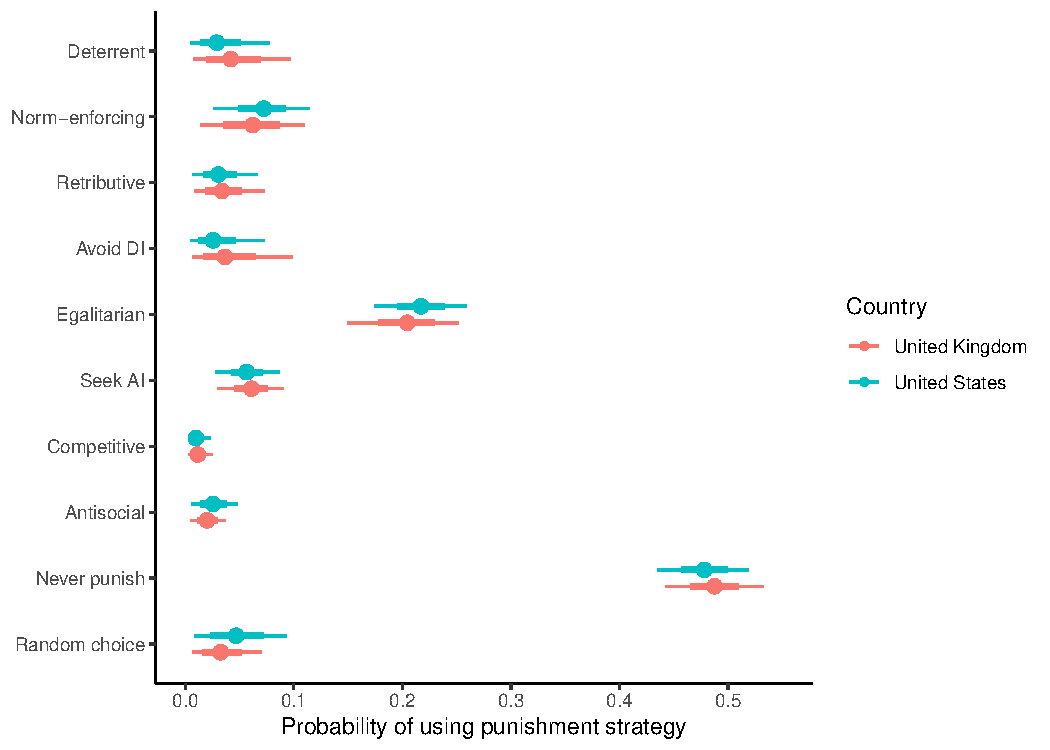
\includegraphics{manuscript_files/figure-latex/plotModel1a-1.pdf}
\caption{\label{fig:plotModel1a}\emph{Posterior estimates of the probabilities of following
different punishment strategies from the Bayesian latent state model fitted to
the full dataset without pre-registered exclusions.} The model assumes an
implementation error rate of 5\%. Points represent posterior medians, line ranges
represent 50\% and 95\% credible intervals.}
\end{figure}

\newpage






\begin{figure}
\centering
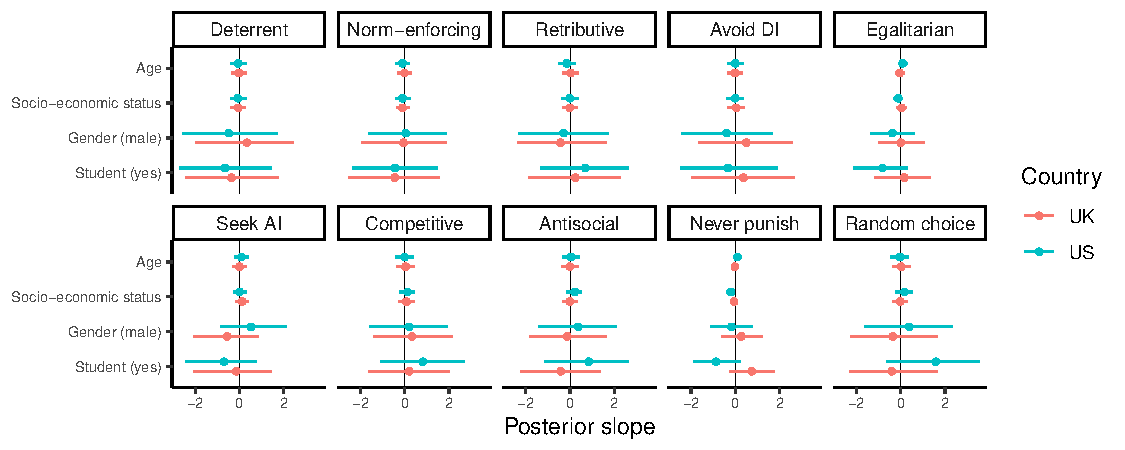
\includegraphics{manuscript_files/figure-latex/plotAllDems2-1.pdf}
\caption{\label{fig:plotAllDems2}\emph{Posterior slopes from models including age,
socio-economic status, gender, and student status, fitted to the subsetted
dataset with pre-registered exclusions.} Each row represents a separate model.
Points represent posterior medians, line ranges represent 95\% credible intervals.}
\end{figure}

\newpage






\begin{figure}
\centering
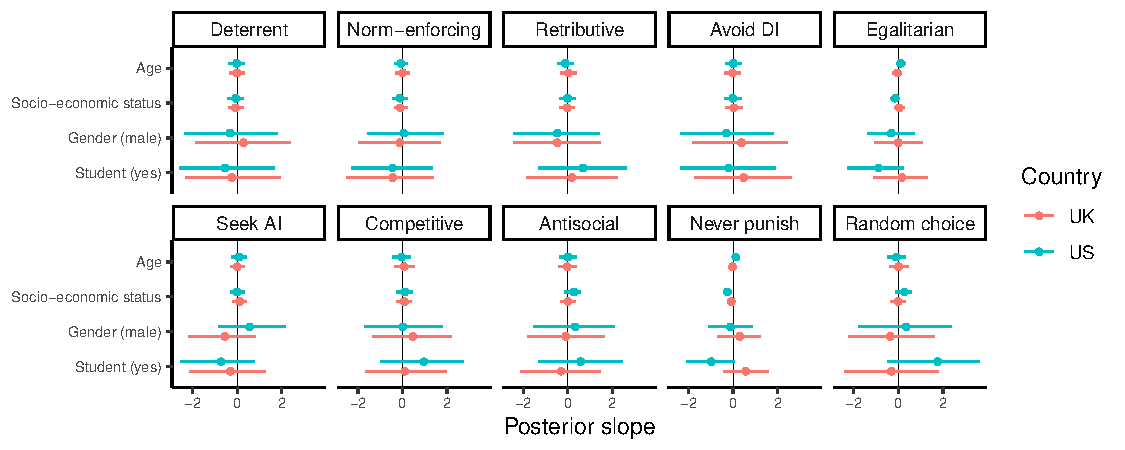
\includegraphics{manuscript_files/figure-latex/plotAllDems1-1.pdf}
\caption{\label{fig:plotAllDems1}\emph{Posterior slopes from models including age,
socio-economic status, gender, and student status, fitted to the full dataset
without pre-registered exclusions.} Each row represents a separate model. Points
represent posterior medians, line ranges represent 95\% credible intervals.}
\end{figure}

\newpage






\begin{figure}
\centering
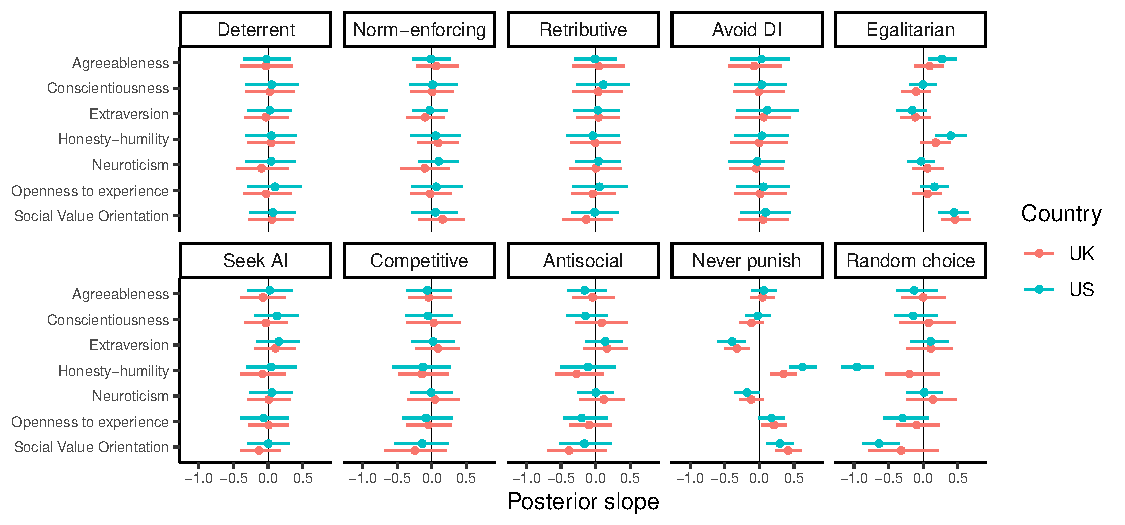
\includegraphics{manuscript_files/figure-latex/plotAllPers1-1.pdf}
\caption{\label{fig:plotAllPers1}\emph{Posterior slopes from models including Big-6
personality dimensions and Social Value Orientation, fitted to the full dataset
without pre-registered exclusions.} Each row represents a separate model. Points
represent posterior medians, line ranges represent 95\% credible intervals.}
\end{figure}

\newpage








\begin{figure}
\centering
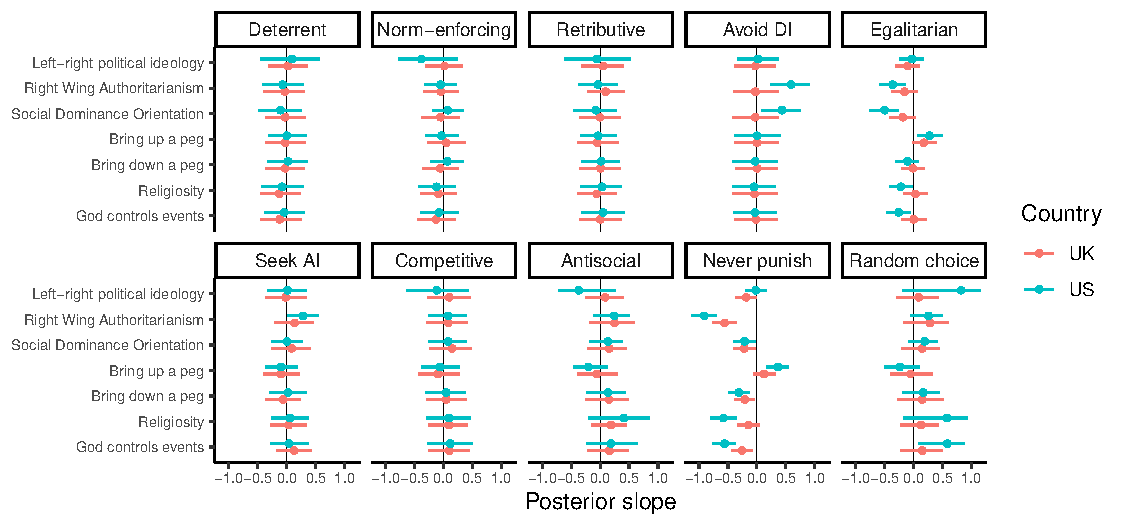
\includegraphics{manuscript_files/figure-latex/plotAllPolRel1-1.pdf}
\caption{\label{fig:plotAllPolRel1}\emph{Posterior slopes from models including political
ideology, views about social inequality, and religiosity, fitted to the full
dataset without pre-registered exclusions.} Each row represents a separate model
aside from Social Dominance Orientation and Right Wing Authoritarianism, which
control for one another within the same model. Points represent posterior
medians, line ranges represent 95\% credible intervals.}
\end{figure}

\newpage





\begin{figure}
\centering
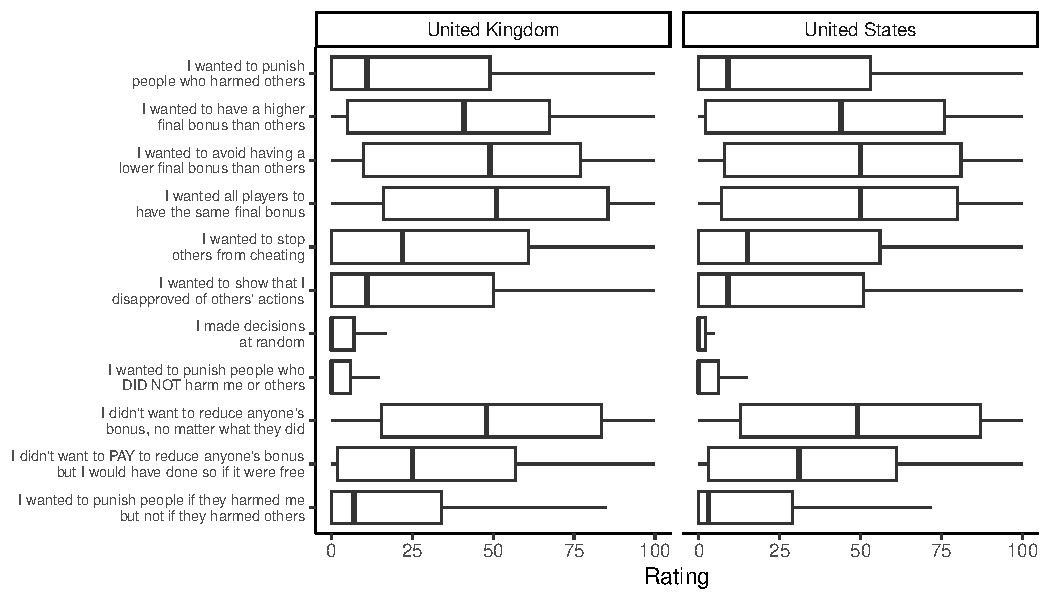
\includegraphics{manuscript_files/figure-latex/plotSliders1-1.pdf}
\caption{\label{fig:plotSliders1}\emph{Boxplots showing the distribution of responses to each
self-report question about the reasons for participants' behaviour in the games.}
Boxplots represent medians and interquartile ranges.}
\end{figure}

\newpage






\begin{figure}
\centering
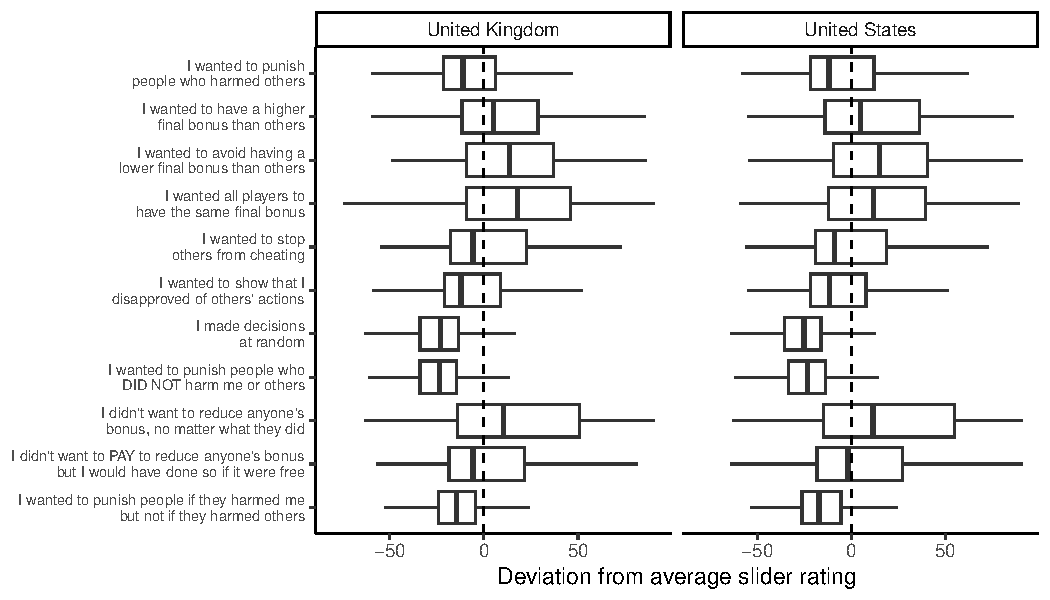
\includegraphics{manuscript_files/figure-latex/plotSliders2-1.pdf}
\caption{\label{fig:plotSliders2}\emph{Boxplots showing the distribution of responses to each
self-report question about the reasons for participants' behaviour in the games,
presented as deviations from participants' average rating across all questions.}
Boxplots represent medians and interquartile ranges.}
\end{figure}

\newpage









\begin{figure}
\centering
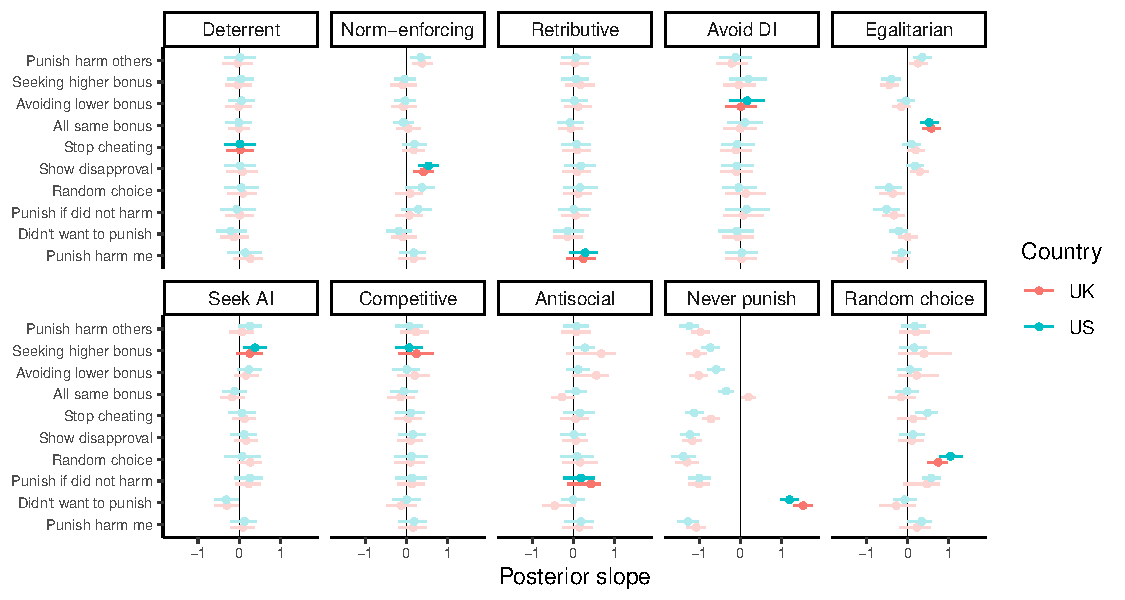
\includegraphics{manuscript_files/figure-latex/plotAllSliders1-1.pdf}
\caption{\label{fig:plotAllSliders1}\emph{Posterior slopes from models including
self-reported strategy usage, fitted to the full dataset without pre-registered
exclusions.} Each row represents a separate model. Highlighted estimates
represent combinations where the self-report slider matched the behavioural
strategy. Each strategy had an associated self-report slider except for the
competitive strategy. Points represent posterior medians, line ranges represent
95\% credible intervals.}
\end{figure}

\newpage



\begin{figure}
\centering
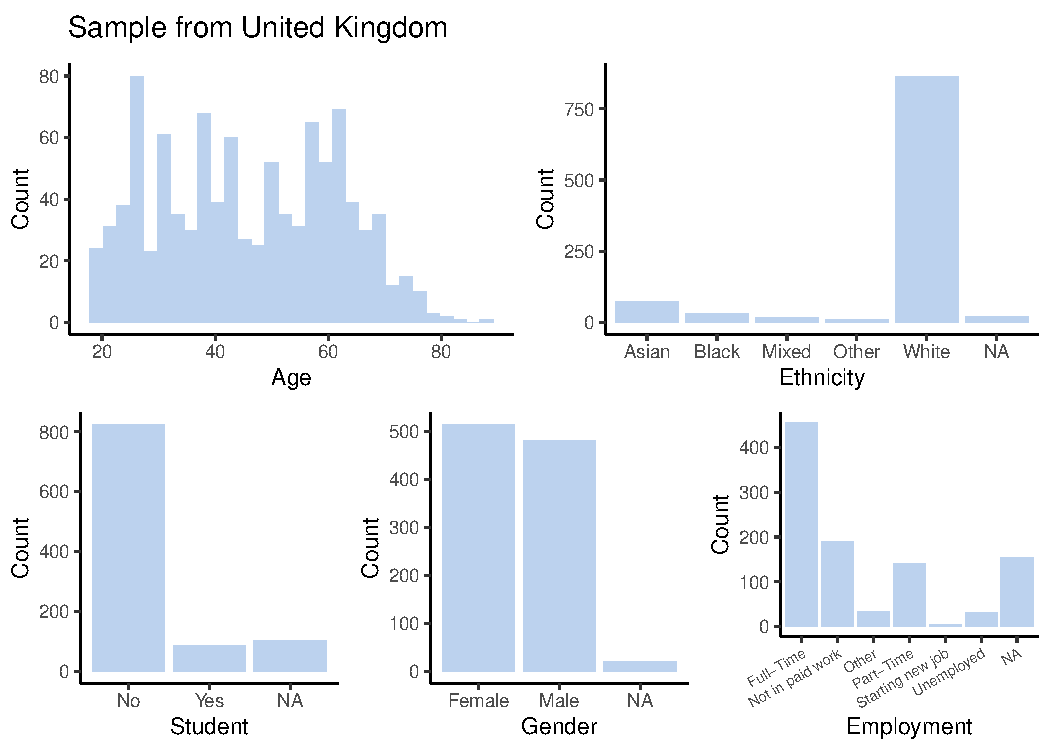
\includegraphics{manuscript_files/figure-latex/plotSampleUK-1.pdf}
\caption{\label{fig:plotSampleUK}\emph{Sample characteristics in the United Kingdom.}}
\end{figure}

\newpage



\begin{figure}
\centering
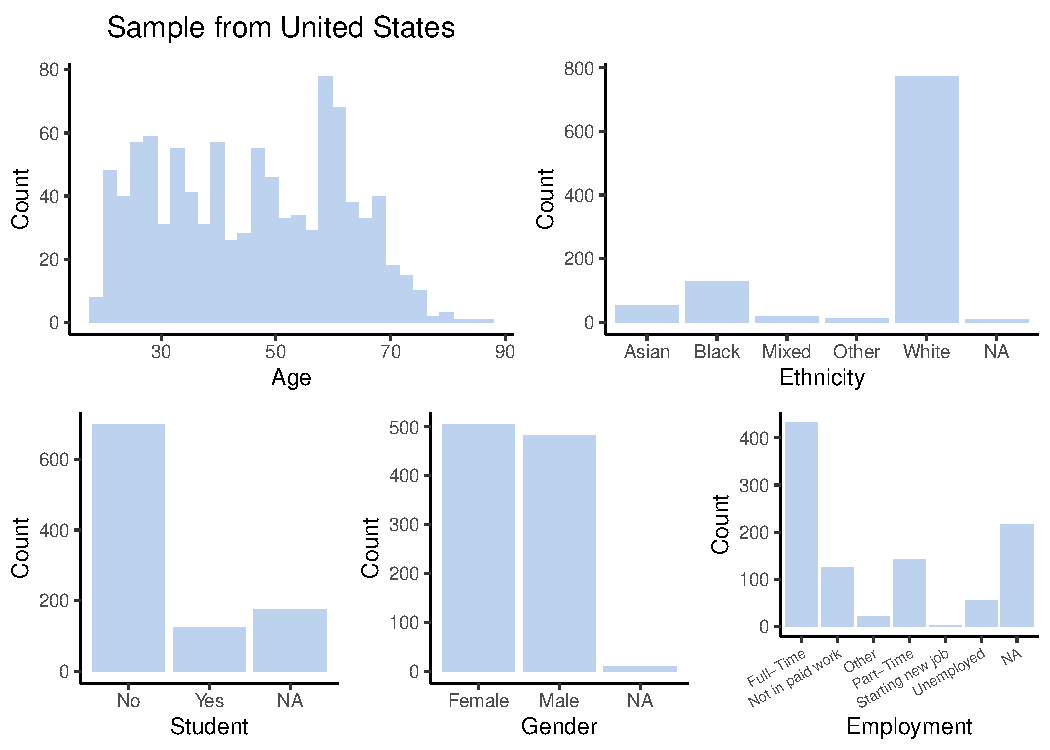
\includegraphics{manuscript_files/figure-latex/plotSampleUS-1.pdf}
\caption{\label{fig:plotSampleUS}\emph{Sample characteristics in the United States.}}
\end{figure}

\newpage




\begin{figure}
\centering
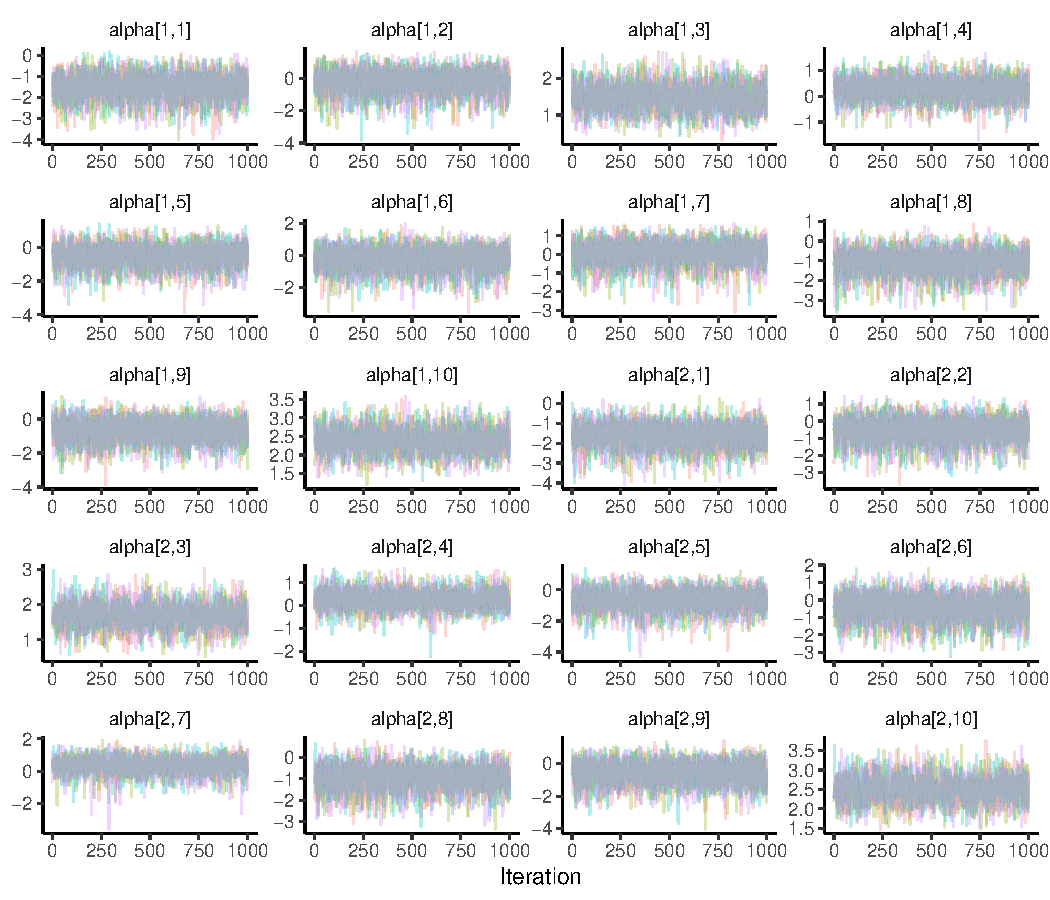
\includegraphics{manuscript_files/figure-latex/plotTrace-1.pdf}
\caption{\label{fig:plotTrace}\emph{Trace plots for parameter values from the Bayesian
latent state model fitted to data with exclusions.}}
\end{figure}

\newpage






\begin{figure}
\centering
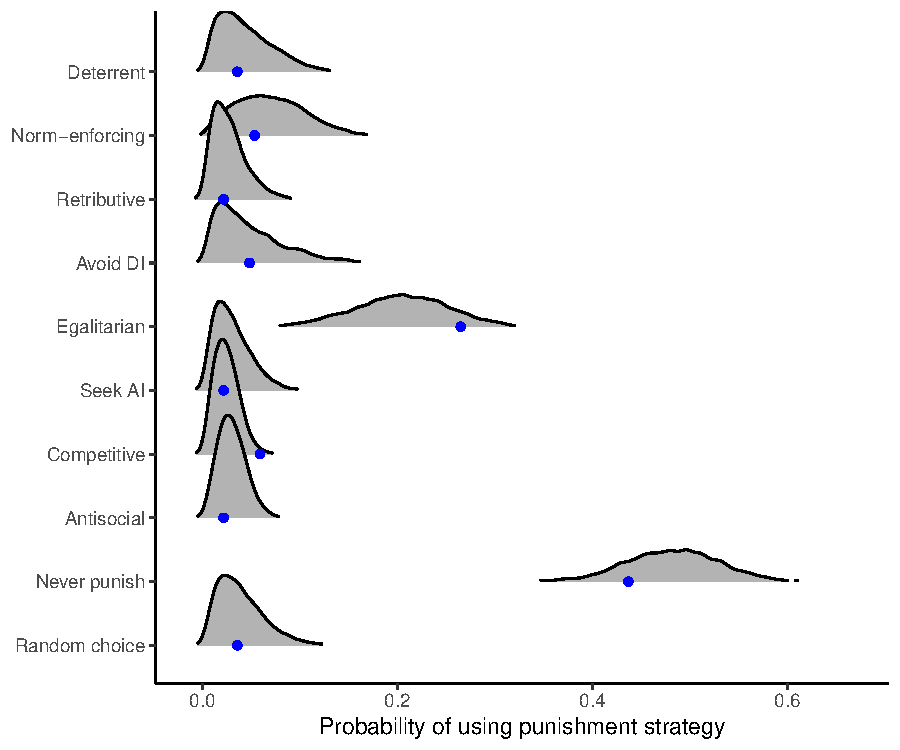
\includegraphics{manuscript_files/figure-latex/plotSim-1.pdf}
\caption{\label{fig:plotSim}\emph{Results of Bayesian latent state model fitted to simulated
data (n = 100) with known strategy frequencies in the population.} Blue points
represent known strategy frequencies, grey densities represent posterior
estimates of strategy frequencies.}
\end{figure}

\newpage

\hypertarget{supplementary-tables}{%
\subsection{Supplementary Tables}\label{supplementary-tables}}






\begin{table}[H]

\begin{center}
\begin{threeparttable}

\caption{\label{tab:tablePatterns}Counts and proportions of the 25 most common patterns
of punitive behaviour across all twelve decisions, split by country. \emph{Binary
strings represent punishment (1) or no punishment (0) in each decision, aligning
with the order of game decision columns in Table \ref{tab:tableStrategies}.}}

\footnotesize{

\begin{tabular}{llcccc}
\toprule
 &  & \multicolumn{2}{c}{\thead{United Kingdom \\ (N = 1014)}} & \multicolumn{2}{c}{\thead{United States \\ (N = 996)}} \\
\cmidrule(r){3-4} \cmidrule(r){5-6}
Pattern & \multicolumn{1}{c}{Explanation} & \multicolumn{1}{c}{N} & \multicolumn{1}{c}{Prop} & \multicolumn{1}{c}{N} & \multicolumn{1}{c}{Prop}\\
\midrule
000000000000 & \textit{Never punish strategy (exact)} & 426 & 0.420 & 447 & 0.449\\
000000001000 & \textit{Avoid DI strategy (exact)} & 67 & 0.066 & 62 & 0.062\\
000000001010 & \textit{Egalitarian strategy (exact)} & 65 & 0.064 & 71 & 0.071\\
000000000010 & Punish when take in Game F & 55 & 0.054 & 49 & 0.049\\
001000001000 & Punish when take in Games B and E & 14 & 0.014 & 11 & 0.011\\
101000001010 & Punish when take in Games A, B, E, and F & 11 & 0.011 & 4 & 0.004\\
100000000000 & Punish when take in Game A & 10 & 0.010 & 2 & 0.002\\
000000100000 & Punish when take in Game D & 9 & 0.009 & 3 & 0.003\\
001000001010 & Punish when take in Games B, E, and F & 9 & 0.009 & 17 & 0.017\\
101000101000 & \textit{Deterrent strategy (exact)} & 9 & 0.009 & 6 & 0.006\\
101010101010 & Punish when take in all games & 9 & 0.009 & 15 & 0.015\\
101000101010 & \textit{Norm-enforcing strategy (exact)} & 8 & 0.008 & 16 & 0.016\\
001000000000 & Punish when take in Game B & 7 & 0.007 & 4 & 0.004\\
001010101000 & Punish when take in Games B, C, D, and E & 7 & 0.007 & 0 & 0.000\\
100000001000 & Punish when take in Games A and E & 6 & 0.006 & 5 & 0.005\\
101000001000 & Punish when take in Games A, B, and E & 6 & 0.006 & 7 & 0.007\\
101010101000 & \textit{Retributive strategy (exact)} & 6 & 0.006 & 5 & 0.005\\
111111111111 & Always punish & 6 & 0.006 & 16 & 0.016\\
000000101000 & Punish when take in Games D and E & 5 & 0.005 & 2 & 0.002\\
000000101010 & Punish when take in Games D, E, and F & 5 & 0.005 & 3 & 0.003\\
101010001010 & Punish when take in all games except Game D & 5 & 0.005 & 2 & 0.002\\
001000101000 & Punish when take in Games B, D, and E & 4 & 0.004 & 2 & 0.002\\
001000101010 & Punish when take in Games B, D, E, and F & 4 & 0.004 & 6 & 0.006\\
101000000000 & Punish when take in Games A and B & 4 & 0.004 & 2 & 0.002\\
101010001000 & Punish when take in Games A, B, C, and E & 4 & 0.004 & 0 & 0.000\\
\bottomrule
\end{tabular}

}

\end{threeparttable}
\end{center}

\end{table}

\newpage









\begin{table}[H]

\begin{center}
\begin{threeparttable}

\caption{\label{tab:tableSliderWordings}Wordings for 11 self-report slider questions
asking participants to report the reasons for their behaviour in the six games.
\emph{Participants were prompted with the following text: ``We would now like you to
answer a few questions about your main motivation in the games. Please answer
truthfully - there is no right or wrong answer and your first answer is probably
best. Please rate the extent to which the following statements apply to your
decisions to reduce or not to reduce other players' bonuses in the games.''}}

\footnotesize{

\begin{tabular}{ll}
\toprule
Slider & \multicolumn{1}{c}{Wording}\\
\midrule
1 & I wanted to punish people who harmed others\\
2 & I wanted to have a higher final bonus than others\\
3 & I wanted to avoid having a lower final bonus than others\\
4 & I wanted all players to have the same final bonus\\
5 & I wanted to stop others from cheating\\
6 & I wanted to show that I disapproved of others' actions\\
7 & I made decisions at random\\
8 & I wanted to punish people who DID NOT harm me or others\\
9 & I didn't want to reduce anyone's bonus, no matter what they did\\
10 & I didn't want to PAY to reduce anyone's bonus but I would have done so if it were free\\
11 & I wanted to punish people if they harmed me but not if they harmed others\\
\bottomrule
\end{tabular}

}

\end{threeparttable}
\end{center}

\end{table}

\newpage



\begin{lltable}

\begin{longtable}{p{6cm}p{11cm}p{3cm}}\noalign{\getlongtablewidth\global\LTcapwidth=\longtablewidth}
\caption{\label{tab:tableSurveyWordings}Wordings for survey questions in the study.}\\
\toprule
Measure & \multicolumn{1}{c}{Wording} & \multicolumn{1}{c}{Scale}\\
\midrule
\endfirsthead
\caption*{\normalfont{Table \ref{tab:tableSurveyWordings} continued}}\\
\toprule
Measure & \multicolumn{1}{c}{Wording} & \multicolumn{1}{c}{Scale}\\
\midrule
\endhead
Demographics & What is your highest level of education? & \\
 & Where would you place yourself on this ladder? Please indicate which number on the rung best represents where you stand at this time in your life, relative to other people in your country & \\
 & Please could you tell us roughly how many years have you lived in your current country of residence? & \\
Big 6 Extraversion & I am the life of the party & 1-7\\
 & I don't talk a lot (reversed) & 1-7\\
 & I keep in the background (reversed) & 1-7\\
 & I talk to a lot of different people at parties & 1-7\\
Big 6 Agreeableness & I sympathise with others' feelings & 1-7\\
 & I am not interested in other people's problems (reversed) & 1-7\\
 & I feel others' emotions & 1-7\\
 & I am not really interested in others (reversed) & 1-7\\
Big 6 Conscientiousness & I get chores done right away & 1-7\\
 & I like order & 1-7\\
 & I make a mess of things (reversed) & 1-7\\
 & I often forget to put things back in their proper place (reversed) & 1-7\\
Big 6 Neuroticism & I have frequent mood swings & 1-7\\
 & I am relaxed most of the time (reversed) & 1-7\\
 & I get upset easily & 1-7\\
 & I seldom feel blue (reversed) & 1-7\\
Big 6 Openness to experience & I have a vivid imagination & 1-7\\
 & I have difficulty understanding abstract ideas & 1-7\\
 & I do not have a good imagination (reversed) & 1-7\\
 & I am not interested in abstract ideas (reversed) & 1-7\\
Big 6 Honesty-humility & I feel entitled to more of everything (reversed) & 1-7\\
 & I deserve more things in life (reversed) & 1-7\\
 & I would like to be seen driving around in a very expensive car (reversed) & 1-7\\
 & I would get a lot of pleasure from owning expensive luxury goods (reversed) & 1-7\\
Social Value Orientation & Please indicate how you would like to distribute money between yourself and the other player & 9 choices\\
Left-right political ideology & Political views are often organised on a single scale from left to right. For example, in the United States, the Democratic Party is described as more to the left and the Republican Party is described as more to the right. If you had to place your political views on this left-right scale, generally speaking, where would you put yourself? & 0-100 slider\\
Social Dominance Orientation & An ideal society requires some groups to be on top and others to be on the bottom & 1-7\\
 & Some groups of people are simply inferior to other groups & 1-7\\
 & No one group should dominate in society (reversed) & 1-7\\
 & Groups at the bottom are just as deserving as groups at the top (reversed) & 1-7\\
 & Group equality should not be our primary goal & 1-7\\
 & It is unjust to try to make groups equal & 1-7\\
 & We should do what we can to equalize conditions for different groups (reversed) & 1-7\\
 & We should work to give all groups an equal chance to succeed (reversed) & 1-7\\
Right Wing Authoritarianism & It's great that many young people today are prepared to defy authority (reversed) & 1-9\\
 & What our country needs most is discipline, with everyone following our leaders in unity & 1-9\\
 & God's laws about abortion, pornography, and marriage must be strictly followed before it is too late & 1-9\\
 & There is nothing wrong with premarital sexual intercourse (reversed) & 1-9\\
 & Our society does NOT need tougher government and stricter laws (reversed) & 1-9\\
 & The facts on crime and the recent public disorders show we have to crack down harder on troublemakers, if we are going to preserve law and order & 1-9\\
Views on social inequality & I would like to bring the people above me on the ladder down a peg or two & 1-7\\
 & I would like to bring the people below me on the ladder up a peg or two & 1-7\\
Religious views & How religious are you? & 1-5\\
 & It is likely that God, or some other type of spiritual non-human entity, controls the events in the world & 1-7\\
\bottomrule
\end{longtable}

\end{lltable}

\newpage




\begin{table}[H]

\begin{center}
\begin{threeparttable}

\caption{\label{tab:tableComp}Proportions of correct answers to comprehension
questions for all six economic games, split by country.}

\begin{tabular}{lll}
\toprule
Game & \multicolumn{1}{c}{United Kingdom} & \multicolumn{1}{c}{United States}\\
\midrule
Game A (AI) & 0.96 & 0.94\\
Game B (Equal) & 0.95 & 0.93\\
Game C (Computer) & 0.95 & 0.95\\
Game D (1:1 Fee-Fine) & 0.95 & 0.94\\
Game E (DI) & 0.96 & 0.94\\
Game F (Third-Party) & 0.95 & 0.94\\
\bottomrule
\end{tabular}

\end{threeparttable}
\end{center}

\end{table}


\end{document}
